  %% LaTeX2e class for student theses
%% sections/content.tex
%% 
%% Karlsruhe Institute of Technology
%% Institute for Program Structures and Data Organization
%% Chair for Software Design and Quality (SDQ)
%%
%% Dr.-Ing. Erik Burger
%% burger@kit.edu
%%
%% Version 1.3.2, 2017-08-01

%TODO da es noch häufiger vorkommen wird, Position der Bilder fixen, aber jetzt mal ehrlich
\chapter{Foundations}
\label{ch:basiscs}
In this chapter, we will introduce the foundations that we are using in my thesis. For each, we will give a short definition and an explanatory example.
\section{Terminology}
\subsection{security relevant data}
The term \textit{security relevant data} as used in this thesis, describes data which should be protected by the system. Security relevant data describes the data that causes harm for user or the system. As an example the security relevant data for a software system may consist of personal related informations, like name, address, credit card, etc. But the security relevant data is from system to system different. The term security relevant data is used in this thesis to describe data that is worth protecting in a system. 
\subsection{Data flow}
\begin{figure}[!htb]
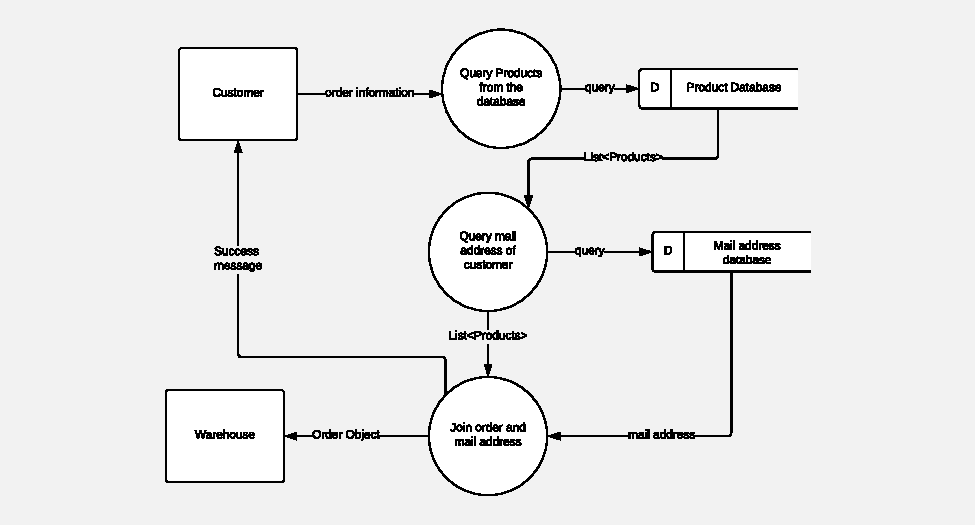
\includegraphics[scale=1]{logos/Simple_Dataflow.pdf}
\caption{Simple data flow diagram for linking an order of different products to a mail address}
\label{fig:simpleDataflow}
\end{figure}
The term data flow is used in different fields of computer science. To name a few examples, data flow is used in software architecture, hardware architecture, networking, etc. We mainly use data flow in our architectural models \\
Data flow describes the way of data through a system. One can imagine data flows like an activity diagram. Each node in the diagram is either a process or an external entity. Processes are operations which processes the data. External entities are users or other systems which request or submit data. The edges between the nodes containing the type of the data passed. Also different data stores (most likely databases) are part of the diagram. These data stores holds different information, like the credentials, and are accessed via a process.\\
\autoref{fig:simpleDataflow} shows the simple process of ordering products and linking them to a mail address. The customer is already authenticated and inserts the order informations. Then the system queries all the necessary informations for the products from the database and adds them to a list. After that, the mail address of the customer is queried and packed in an object together with the product list. This object is then send to the warehouse and the customer is presented a success message. Later, the warehouse will collect the products and pack them in a delivery, but this is not a part of the diagram. For the sake of simplicity, eventual errors aren't modeled. 

\section{Palladio Component Model}
\label{sec:PCMIntro}
%The Palladio Component Model (PCM) is an ADL that is used to model component based systems. The 
\subsection{Component based systems}
%TODO component based systems erklären 
Component based system are systems that consist out of components. Each component in a system is usually designed to fulfill one functionality, like connecting to a database, handling the user input, etc. It is possible that a component consists of multiply component. In such a composite component, each component also handles a single task. This allows to split larger tasks into smaller ones and assign each of them to a single component. This allows to reuse components that are designed to handle general tasks, like formatting data to a String.The definition of a component is that a component provides or requires an interface. The provided or required interfaces are used for communication between the components. Each of the interfaces is clearly defined. The components are chained together to a system using the interfaces. The main strength of the component based systems are the modularity by design. As simple example is shown in \autoref{CBS_simple}. In the model a simple oline shop is shown. As shown, there is a component for managing the warehouse, a component for handling the business logic e.g. selling products and a component for the user interface. In this component based system the  user interface is used by both customers and employees. Usually each of the components consists of different components for th different tasks. 
%TODO bildchen malen
\begin{figure}
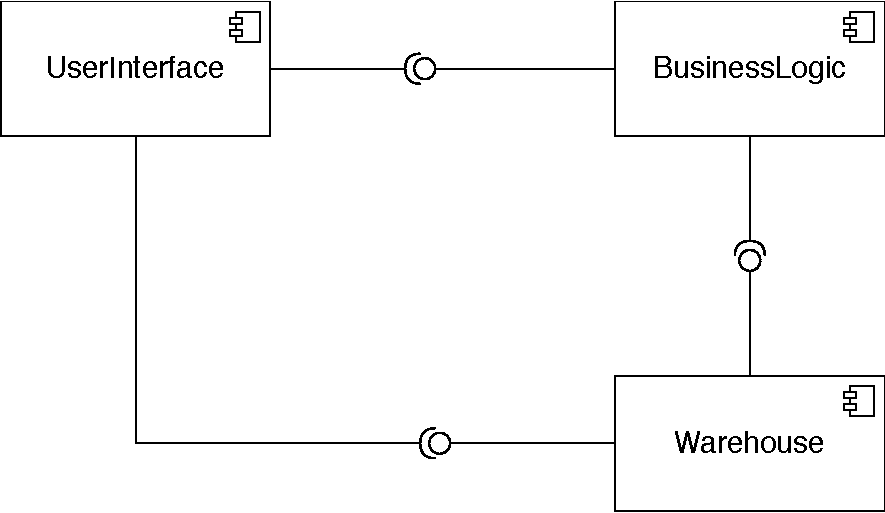
\includegraphics[scale=.8]{logos/SimpleCBS.pdf}
\caption{A simple component based system}
\label{CBS_simple}
\end{figure}
\section{Data Centric PCM}
\subsection{Concept}
The Palladio Component Model (PCM) is an architecture description language (ADL) , that allows more than only modeling a system. The strength of PCM is compute performance predictions for the modeled system \cite{PCM}. 
%TODO hie rnoch genauer formulieren
A PCM model consists of four different models, each of them encapsulate their specific design knowledge and the models build on each other. After the system is complete, an architect may compute different predictions how the system will perform when it is deployed. The predictions are for cost, reliability, performance and maintainability. In the following, we will explain the individual models and their encapsulated design knowledge in detail. \\
First of all, for each model a role inside the PCM is assigned, which will be explained in detail later. Each of this roles conserve their design knowledge in a specific model which is used by the next role. The hierarchy of the different roles , from top to bottom, is:
\begin{itemize}
\item \textbf{Component Developer}\\
The component developer specifies and implements the component. Furthermore, s/he has to provide additional information, that will be used for the predictions, PCM is able to compute. The resulting model is called \textit{repository model} and is used by the system architect.
\item \textbf{Software Architect}\\
The system architect builds the system using components. S/He connects the different components provided by component developers to a fully functional system. The resulting model is called \textit{system model} and is used by the system deployer.
\item \textbf{System Deployer}\\
The system deployer decides  how the system is distributed between the available resources. 
This role creates two resulting models. First, the \textit{resource model}, in which the resources characteristics, for example transfer rate. Second, the \textit{allocation model}, in which the allocation of the different resources to the different parts of the system is conserved. These models are used by the domain expert.
\item \textbf{Domain Expert}\\
Domain experts creates the \textit{usage model} for the system. This describes user behavior. Also they specify the user workload. This workloads can be open or closed. In the closed case, a finite number of user interact with the system, in the open case the domain expert specifies the user arrival per time slice.\\
As the domain expert is the last role in the chain, the models aren't used by another role. With the addition of the usage model the creation of the system model is complete.
\end{itemize}

After all the different models are created, a prediction may be computed and without a line of code is written and the architects can see if there are flaws in the architecture. The PCM models are more than just a system model. A lot of domain knowledge is encapsulated in the resulting models. The result are more a simulation for the upcoming system than a system model.
\subsection{Meta model extension for data centric PCM}
\label{MMext}
% Meta model erklären
In this section, we are going to explain the meta model extension to the PCM provided by Seifermann \cite{MMextension}. The extension is lightweight. It aims to embed data flows in an already existing PCM model.\\ 
In the current state of PCM, it is not possible to model data flows. Therefore Seifermann created a meta model extension. The meta model extension is called data processing. \\
The meta models extends the Service Effect Specification (SEFF) for a component in the repository model. SEFFs are similar to UML activity diagrams. Like Activity diagrams, SEFFs specify the observable behavior for a system, in the case of PCM SEFFs specify the observable behavior for a component. SEFFS are used to model different types of actions. These actions holds various information about the systems performance and are chained together to create a sequence of events to model the (observable) behavior of a specific component.\\ The meta model extension is specially for these SEFFs. The main goal for this meta model extension was to model data processing.  For each action in a SEFF an operation may be defined that specifies the data processing for this action. The operations model different types of manipulation of data. All SEFFs chained together in model already create a model similar to an activity diagram. For each activity a operation that processes data is specified. With this operations chained together it is possible to create a data flow for the model. 
\section{Goal-Question-Metric approach}
\label{GQM_Expl}

%TODO related work hier hinein
\chapter{Related work}
After the foundations were presented, we discuss here the related work.  First, we present the work that was the basis for further work on this paper.
%TODO grundlegender Aufbau, es wird klar gemacht, dass wir eine procedure für das Erstellen von case studies erstellt haben. 2 Teile: 1) Erstellen der CS (Runeson, Höst) und die Sicherheitsansätze (Non_influence, Mclean, usw) -> es gabe eine publication die beides vereint hat, evered Bögeholz !!!

After the contributions of the thesis have been evaluated, they are placed in the context of related works. First, it has to be said that related work for the kind of case study we created was hard to find. Case studies are an acknowledged procedure mainly in the fields of sociology, philosophy, law, etc. For this fields, the case study method is documented well. The type of case study that we are going to create shows some similarities with case studies that were created in the previously mentioned fields. Nevertheless, the discrepancy between computer science and the classical fields for case studies, is too great. Only fundamental methods could be adopted by the method. Such methods includes, for example, to use two sources of data \cite{cs2sources}. In the field of computer science, case studies are mostly used to give an overview of certain topics, e.g. how different challenges in software engineering were tackled. Sometimes there are used to verify the applicability of different approaches, like UMLSec \cite{UMLSecCS}. The only publication that roughly outlines the creation a case study for a software system, was the one from Evered and Bögeholz \cite{CaseStudyAndAccessrigths}. In this publication, the both authors describe briefly the creation of a case study on a much smaller system than we performed our case study on. The main goal of their publication was to define good access rights in component based systems by using their structure. We have adopted the introduced criteria of Evered and Bögeholz \cite{CaseStudyAndAccessrigths} and have included them in our evaluation as a measurement for good access rights. Further, the author described briefly the creation of a case study. In their publication, the defined first the data than the access rights and then went right to evaluation. In their work this was enough because the main aim of their work was to evaluate the different types how access rights may be added to a running system. In contrast to Evered and Bögeholz, the aim for our case study was to be used in a data-based privacy analysis. Therefore we used their approach as a basis for ours. We require a specific system model and the existence or the deductibility of use cases to ease up the later validation. Further, in contrast to Evered and Bögeholz, we want to use the created case study in another setting. Therefore we added the definition of scenarios and the definition of the type of data processing for each component and each role. All in all, we say that Evered and Bögeholz have given us a good starting point for our method and we have expanded theirs.\\ We lloked further but could not find any other fitting publications that may address our matter. We found a lot publications that adresses different case studies but none with the same or similar aim as our method.
\chapter{Procedure}
\label{ch:method}
% was werde ich in diesem chapter vorstellen ?
%Fertig

%TODO wir stützen uns auf privacy analysen auf access rights
In this chapter we are going to present a procedure to create a case study that can be used to evaluate a data-based privacy analysis. The privacy is defined by access rights. We will describe the procedure step by step and the places where the case study will be evaluated. During the process, the case study is evaluated based on two aspects,the quality of the access rights and the covered information flow classes. Overall, the resulting case study consists of an extended system model. The extensions include the access rights and the added data flows. \\
First, we give a brief overview over the procedure shown in \autoref{overview_cs_rep}. After that each step will be explained in detail. \\ 
The procedure consists of seven consecutive steps. First the current state of the system is reviewed, secondly the necessary elements for the requirements are extracted. Thereafter the fulfillment of the requirements is reviewed and the required system extensions are defined in the next step. Afterwards, the access rights are evaluated and the results are stored in a milestone. Then scenarios for the system are defined. In the final step, the information flow classes covered by the scenarios are evaluated. Finally, it is decided whether the case study is sufficient for the intended use. 
% layout des chapters.
\section{General procedure for the creation of a viable case study}
\label{cs_overview}
\begin{figure}
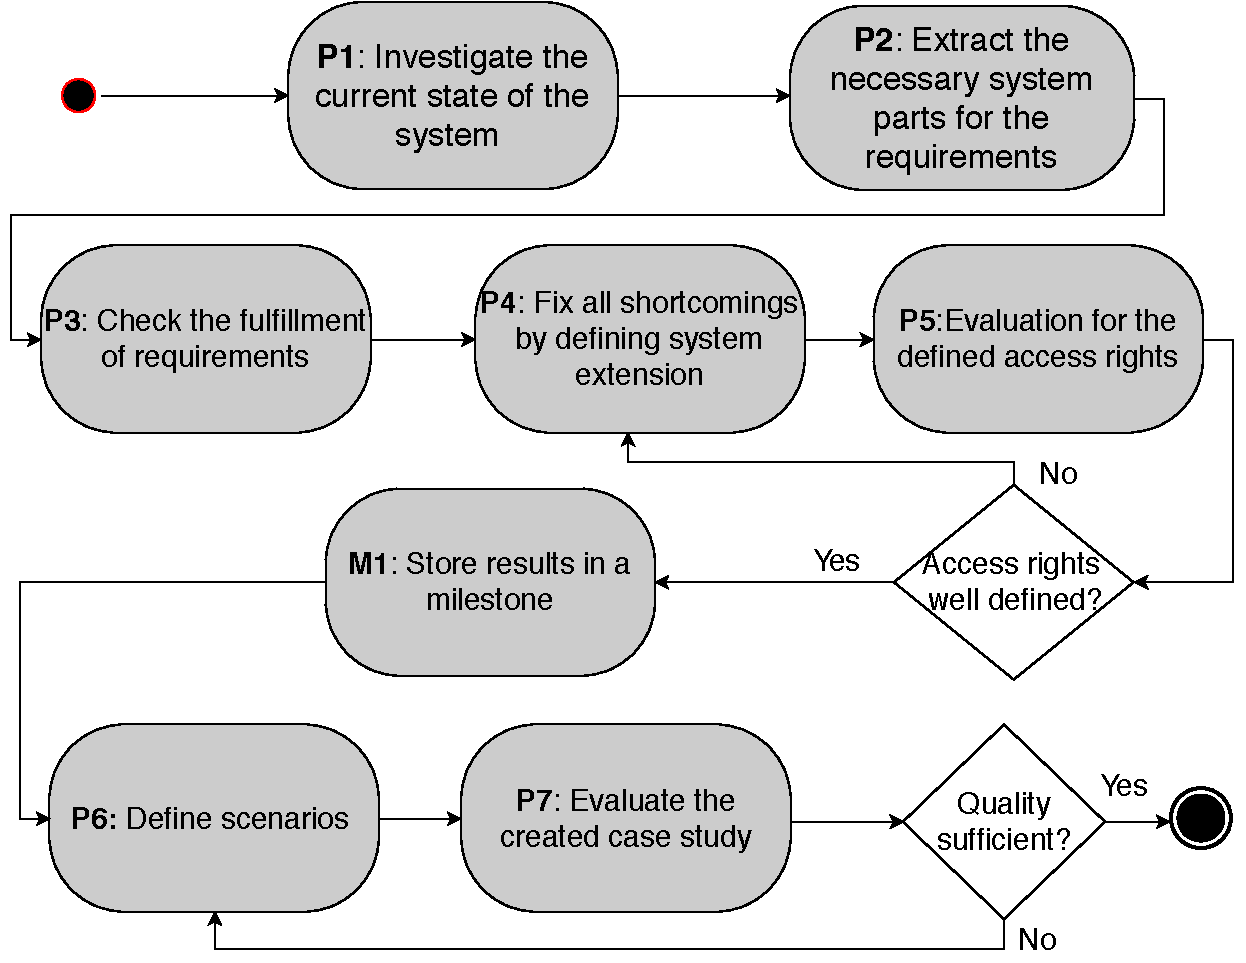
\includegraphics[scale=.7]{logos/Procedure.pdf} 
\caption{General overview over the procedure for creating a viable case study}
\label{overview_cs_rep}
\end{figure}
Here we describe the procedure for creating a case study. An overview is shown in \autoref{overview_cs_rep}. We cover the steps P1-P7 that are necessary to create a case study. We further explain places when the evaluations are conducted.  \\
% erster Schritt
The first step is to decide whether it is worthwhile to prepare a case study based on the system under investigation. This is decided by reviewing the current documentation. The goal is to   
%TODO das es mehr gibt al eine erste Idee oder ein Konzept (?) -> eventuell schon Systemmodelle, use cases, sequence diagrams etc
% zweiter Schritt + dritter schritt
In a second step, six requirements for creating a case study are introduced (see . The first requirement is that the system is modeled as a component based system or components can be derived from the current documentation of the system. The second requirements is the definition of use cases. The third requirement is to identify the data in the system and identify which of the data is security relevant. The fourth requirement is the definition of user roles in the examined system. The fifth requirement is definition of access rights between (security relevant) data and the user roles. The access rights can either be generated from the previous requirements or extracted from the documentation. The sixth and last requirement is the identification or definition of the different types of data processing. Furthermore, for each component it is either defined or identified which data is processed as in the individual component.\\
%dritter Schritt
In the third step, the current fulfillment of requirements are analyzed and collected in a summary. Usually there are shortcomings. If there are none, the next step can be skipped.\\  
% vierter Schritt
In the fourth system extensions for the missing parts of the requirements are defined. \\
%
%TODO wa spassiert wenn die access rights nicht gut sind ? -> zurück in den vorherign Schritt
In the next step, the evaluation for the the access rights is conducted.\\
After the evaluation is done and the results are sufficient, the milestone is reached. All necessary parts of the system are present, so that a case study can be created. If the results are not sufficient the procedure iterates back to the fourth step. %Iterationback to P4
% fünfter  Schritt\\
% sechster Schritt
In the sixth step, scenarios are defined, from which data flows are derived. Finally, the data flows and the access rights are added to the system model.\\
In the seventh step the covered information flow classes are evaluated. Then it is decided if enough information flow classes are covered for the planned use of the case study. If not, the procedure iterates back to the sixth step. Otherwise, the procedure is concluded and the case study is created. The case study finally consists of the system model extended by data flows and the access rights.
%TODO ab ie rmorgne weitermachen !!!!!
\section{P1: Investigate the current state of the system}
%Fertig
Before the process is started, a first glance at the present system is taken. This first glance is taken to decide whether it is worthwhile to start the process. It is checked if the system is sufficiently defined in \textit{width} and \textit{depth}. \textit{Width} checks how many different system models are already defined. \textit{Depth} checks how detailed each model is defined. The outcome is system dependent. For example, it could be important how much work one is willing to do before starting the process. The idea behind this step is to decide beforehand if the system is in a state where it is more than just a bare concept and the case study can be constructed with reasonable effort.
%TODO requirements fertig 
\section{P2: Extract necessary system parts for the requirements}
\label{cs_req}
The second step in the procedure is to extract the corresponding elements or definitions from the system for each requirement. Altogether, six requirements are necessary for the creation of a viable case study.
\paragraph{R1: Modeled as component based system}
%fertig
The first requirement is that the system is modeled as a component based system or it is possible to derive a component based system from the current state. The allows to use all benefits that a component based systems has and make it much easier to construct a case study. Firstly, in component based system there are well defined interfaces. These interfaces defining points in the architecture where data is transmitted. This ease up the creation of data flows, because one can directly identify where the data is processed. Secondly, component based systems are easy to extend. Therefore, it is not that complex to add missing elements to the model. Thirdly, the component based structure enables modularity. So it is relatively easy to just took an excerpt and take a close look on just this excerpt. All in all combined, component based systems excel in their modularity and their clear defined interfaces, that ease up the creation of a case study.
\paragraph{R2: Definition of use cases}
%Fertig
The second requirement is the definition of use cases in the system or it is possible to derive use cases from, for example, the documentation. This allows to get a good idea how the different users are going to interact with the system. Further, the use cases give a basic idea of the general interaction with the system.

\begin{table}
\begin{tabular}{|c|c|}
\hline 
\multicolumn{2}{|c|}{Requirements} \\ 
\hline 
R1 & component based system \\ 
\hline 
R2 & Definition of use cases \\ 
\hline 
R3 & Security relevant data \\ 
\hline 
R4 & Definition of user roles \\ 
\hline 
R5 & Definition of access rights \\ 
\hline 
R6 & Definition of the type of data processing in the components \\
\hline
\end{tabular} 
\label{req_over_sec}
\caption{An overview over all the requirements for the creation of a case study.}
\end{table}
\paragraph{R3: Existence of security relevant data}
%fertig
The third requirement for a viable case study is the existence of security relevant data in the system. If there is no critical data in the system, the entire case study that is created to verify the protection of security relevant data is pointless. The definition of security-relevant data is highly dependent on the system under investigation. This means for each system and each context there are other data that is considered security relevant, therefore a lot of domain knowledge is required to identify the data. Breier \cite{assetValue} introduced a basic approach to valuate assets. The basic idea of the approach is to value the various assets in terms of their priority within the system. 

\paragraph{R4: Existence of different user roles}
The fourth requirement for the case study is the definition of user roles, in the following briefly roles, for the system. Roles are used to model different types of user for a system. Each role maps to one type of user. Roles are used to model the different users that are interacting with the system. Different roles uses on different data inside the system. For example the security relevant data mentioned in R3. The roles depend heavily on the system being studied. Each system defines different roles. For each system under investigation the use cases (R2) are a good source of informations. One can use business processes \cite{rolesBusiness} to identify roles in a system.
\paragraph{R5: Definition of access rights}
%fertig
The fifth requirement is the definition of access rights. For the definition of access rights, we use the fine-grained, higher level form proposed by Evered and Bögeholz \cite{CaseStudyAndAccessrigths} in contrast to the familiar used read/write semantics. For this step, we assume the system is in a correct state. 
 The access rights are define on the basis of the current state of the system. As already mentioned, each component has a clearly defined interface. These interfaces are used for communication with other components. This structure is used to define a higher level, finer grained form of access control. For each component and each role, the access rights for the data types in the component are defined individually. The access rights are stored in a matrix, the so called access control matrix (ACM). In \autoref{ACMexplained} an minimal ACM is shown to get a better idea of the concept. The matrix shows that the role \textit{Employee} in the component \textit{Usermanager} has full access to username. Also it is shown, that the same role in the same component has no access to the password. It may happen that data is the combination of different data types. In this case, the more restrictive access rights applies. To clarify this, if the employee tries to access a (\textit{username, password}) tuple, s/he is granted no access to the tuple.

\begin{figure}
\begin{tabular}{|c|c|}
\hline 
ACM & Usermanager \\ 
\hline 
Employee &  
\begin{tabular}{c}
username: fullAccess \\
password: noAccess
\end{tabular}
\\ 
\hline 
\end{tabular} 
\caption{Reduced ACM to the show the concept.}
\label{ACMexplained}
\end{figure}

\paragraph{R6: Definition of type of data processing in the components}
In the sixth requirement the type of data processing for each data type in each component is defined. As the the requirement R5, the necessary elements for this requirement may be derived from previous ones, namely R1, R2 and R3. In R1 ensures that the system is modeled as a component-based system. With R2 (definition of use cases) and R3 (security relevant data) it is possible to identify how which data is processed. The different processing types are described through different operations. The various operations describe how and which data is processed in a specific component. Each operation has one more inputs and produces one or more outputs. The  operations needed are highly system-dependent. Operations could describe the transmission of data, processing of user inputs or operations used in the relational algebra. The identified operations are stored in an operations matrix (OpM). In this matrix, for each component it is stored with which operations data can be processed.
In \autoref{opm_expl} an excerpt of an OpM is shown. As one can see, in the component \textit{User interface} it is only possible to transmit the login data to other components.

\begin{table}
\begin{tabular}{|c|c|}
\hline 
 & Login data \\ 
\hline 
User interface & transmit \\ 
\hline 
\end{tabular} 
\caption{A simple example to showcase an OpM.}
\label{opm_expl}
\end{table}

\section{P3: Check fulfillment of requirements}
\label{cs_check}
%fertig
In this step the current state of requirements is reviewed. The best case is, that all requirements are fulfilled. If this is the case, one can skip the next step. If it is not the case, create a summary of all shortcomings for the fulfillment of requirements in the system. After the first two steps of the procedure are done the usual case is that some of the requirements are not fulfilled. It may even happen that for some requirements are no elements present in the system. The review of the shortcomings is important to outline which parts of the system are vague. Vague in the context of the thesis means that some elements (e.g roles, access rights) are not well defined. To give an example, it may happen that roles are just mentioned but a clear definition of the role is missing. This summary of shortcomings may also show parts where the model is not well defined. This may lead to an improvement of the model in the next step. After the summary is complete, the procedure moves to the next step. The summary is done due to two reasons. Firstly, to get a comprehensive overview of the current state of the system and secondly, to enable a division of tasks. The second reason is that you get an overview of the big picture and define possible system extensions not as soon as a shortcoming is encountered but with the big picture in mind. This ensures that system extensions are defined in the context of the whole system.

\section{P4: Fix all shortcomings by defining system extensions}
\label{cs_cocome_ext}
%fertig
In the previous step, a summary of the shortcomings in the system was created. In this summary, all system components that stand in the way of fulfilling the requirements are stored. In this step, the system extensions are defined to fulfill all requirements. When defining system extensions, the first step is to derive the needed extensions from the documentation.  In the case, the documentation isn't clear or it is not possible to derive extensions for the shortcomings, the option left is to define the system extensions to the best of your knowledge. This is sometimes necessary, but there are some dangers involved. It may happen that the resulting case study is less realistic and therefore provides less satisfying results, when used in a later analysis.
\section{P5: Evaluation of the access rights}
In this part of the procedure, the access rights are evaluated. The evaluation follows a GQM-plan, shown in \autoref{GQM_AR}.
  %TODO GQM plan
The access rights are evaluated based on seven criteria presented by Evered and Bögeholz \cite{CaseStudyAndAccessrigths}. We divided the seven criteria in three categories: \textit{specification}, \textit{comprehensibility} and \textit{implementation}. \textit{Specification} how the access rights are defined. \textit{Comprehensibility} evaluates how well access rights can be understood by others. \textit{Implementation} evaluates the way the access rights are embedded in the code. It may not be possible for all systems to evaluate all seven criteria. The seven criteria are:
\begin{itemize}
\item Concise : Access rights should be precise and simple.
\item Clear: At first glance one can see what the access rights state.
\item Aspect-oriented: The access rights may be used in different contexts
\item Need-to-know: each role only should have the absolute necessary informations
\item Positive: Each right to data has to be given specifically to each role.
\item Fundamental: The access rights are realized inside the code 
\item Efficient: The overhead caused by the checks of the access rights is reasonable.
\end{itemize}
The evaluation is done in a checklist manner. For each criterion it is checked whether the system fulfills the criterion or not.\\
After the evaluation of the access rights is done, the results are analyzed. If sufficient criteria for the purpose of the case study are fulfilled, the current state of the system is considered correct. If the results are unsatisfying, the procedure moves back to the previous step P4. Otherwise the milestone is reached. The system is sufficiently defined so that is possible to add data flows and create a case study.
%TODO evaluation done -> deckel alle vorherigen schritte und gehe zum nächsten nasonstne gehe eine schritt zurück und evaluiere neu
%TODO sagen dass alle bisherigen definitionen zusamengesammelt werdne und der aktuelle Stand in eine EMilenstein gespeichert wird
\begin{figure}
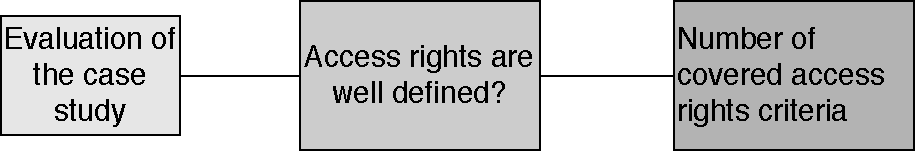
\includegraphics[scale=.6]{logos/GQM_accessrights.pdf}
\caption{Overview of the evaluation of the access rights.}
\label{GQM_AR}
\end{figure}
\section{M1: Store the results in a milestone}
After the evaluation results are sufficient, the current state of the system is stored in a milestone. This includes all definitions made for the each requirement.
\begin{itemize}
\item R1: The system model.
\item R2: Use case diagram, definition for each use case.
\item R3: The data types and the examination, which data is security relevant.
\item R4: The different user roles.
\item R5: The created ACM.
\item R6: The created OpM.
\end{itemize}
\section{P6: Definition of scenarios}
After the milestone is reached, scenarios for the case study are defined. Scenarios are a concrete characteristic of a use case or a concrete characteristic of an interaction with the system. The scenarios are defined taking into account requirements R2, R3, R4 and R6. R5 is omitted in order to reduce the bias of the system architects that not only scenarios are created that are consistent with the access rights. The main part of this step is to transform the created scenarios into data flows that are later added to the model. We will provide a procedure how to add data flows to the model. This is done step-by-step. The defined scenarios serve as the basis for the transformation. To realize the transformation three successive steps are needed. \\
% Komponenten des scenarios
In the first step, the components that are needed to realize the specific scenario are identified. Then these components are collected and added to a reduced model.
% Interfaces zwischen den Komponenten und deren datentypen
In the second step, the reduced model is analyzed. The aim of the analysis is to map data and the respective type of processing to components. Then the data flows can be created and added to the reduced model. 
In an last optional step, the reduced model is added back to the originally model. This can be done,so all data flows are available in the original model. \\
This procedure is repeated for each scenario. 
After that, the access rights are also added to the component model. The structure of the access control matrix is used. For each component, the respective access rights of a role to the data types of a component are added to the respective components. After this is done, the definition of the scenarios is complete and the added data flows can be evaluated.
\section{P7:Evaluation of the covered information flow classes}
The last step, is the evaluation of the defined scenarios for the system. The scenarios are evaluated on the basis of the information flow classes covered, which may differ according to the objective or use of the case study.  The evaluation follows a GQM-plan. The plan is shown in \autoref{GQM_infoflow}.
We propose to use Non-influence \cite{Noninfluence} and the included information flow classes to evaluate the scenarios. Non-influence consist of the two part: non-interference and non-leakage. Non-interference describes, that in a program flow inputs of high users do not influence the output for low users. Non-leakage describes that it is not possible to observe if a specific action in the system has taken place.\\
non-interference and non-leakage are covered by  the following four information flow classes:
\begin{itemize}
\item No illegal information flow:
\item No information flow from high to low:
\item No direct information flow:
\item No observable information flow:
\end{itemize}  %
\begin{figure}
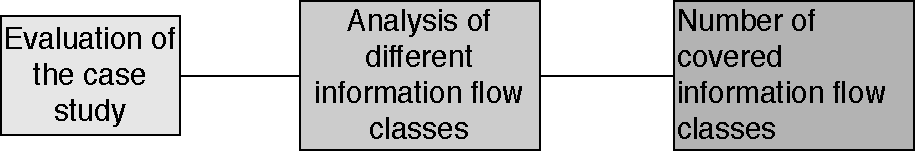
\includegraphics[scale=0.6]{logos/GQM_infloFlow.pdf}
\caption{Overview over the GQM plan for the evaluation of the added data flows.}
\label{GQM_infoflow}
\end{figure}
\section{Conclusion of the procedure}
After the second evaluation is conducted, it is necessary to decide if the coverage of the information flow classes are sufficient for the goal of the cases study. If so, the procedure is finalized and the case study is created. Otherwise, the procedure moves back to the P6.\\ The created case study in the end consist of the system model extended with data flows and the ACM.
%\section{Evaluation of the case study}
%\label{cs_evaluation}
%In his step the evaluation the created case study is presented. The evaluation aims to verify if the created case study is usable for data-based privacy analysis. The evaluation follows a GQM plan \cite{GQM_Intro}. The idea of a GQM plan is to split the evaluation into three parts. First, a goal for the evaluation is defined. In the second step, questions are defined. The answer to this question indicates if the defined goal is reached. In the last step, metrics are defined. These metrics allows to answer the previously asked question.\\
%The evaluation validates the created case study. It is evaluated whether the case study is suitable for a data-based privacy analysis. The evaluation is embedded in an GQM plan. The plan is shown in \autoref{fig:GQMPlan}\\
%
%\begin{figure}
%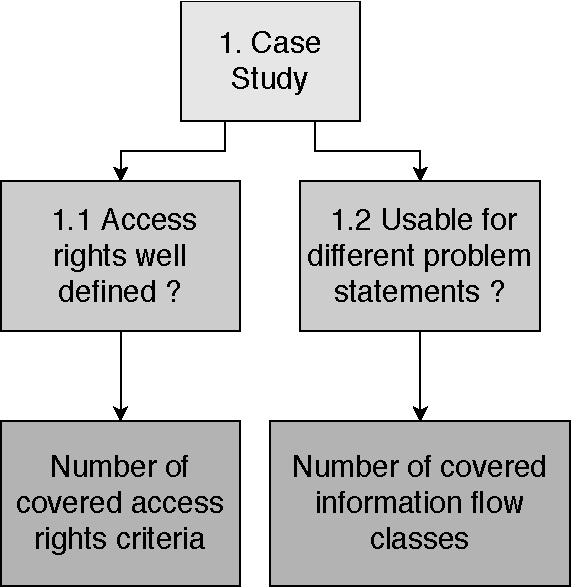
\includegraphics[scale=.8, origin=c ]{logos/GQMPlanGen.pdf}
%\caption{The GQM plan for the evaluation.}
%\label{fig:GQMPlan}
%\end{figure}
%
%The goal is to verify if the created case study is usable for a data-based privacy analysis. To verify this, we defined two questions.
%\begin{itemize}
%\item Are the access rights well defined ?
%\item Are different information flow classes are covered ?
%\end{itemize}
%As a metric for the first question we use a checklist. Evered and Bögeholz \cite{CaseStudyAndAccessrigths} defined seven criteria for good access rights. Not all surveyed systems allows to check the seven criteria: concise, clear, fundamental, need-to-know, efficient, aspect-oriented and positive. Therefore it is case dependent which criteria are applicable. For each selected criterion, the system then checks whether the access rights meet these criteria. After that, based on the fulfilled criteria, it can than be decided if access rights are defined well.\\
%The metric for the second question is also a checklist. To verify the question different classes of (illegal) information flows are defined. Possible information flows classes are that no information flows from higher security levels to lower ones, no direct information flow between different users, etc. Then it is checked for each information flow class whether the case study created expresses it. After that, based on the included information flows, it than can be decided, if the case study covers the desired number of different information flow classes.

\chapter{Analysis of CoCoME}
\label{ch:cocome}
%TODO done
In this chapter we are starting to apply the procedure described in \autoref{ch:method} to CoCoME. The procedure is applied up until the milestone is reached, as seen in % neues bild in dem alle snach dem milestone ausgegraut ist
First we describe CoCoME briefly. Then the steps P1-P5 of the presented procedure are carried out. First we briefly examine the current state of CoCoME, then the system parts necessary for the requirements are identified and/or extracted from the documentation. After that, a summary of the shortcomings is created and in the next step the identified shortcomings are eliminated by defining system extensions. The defined access rights are then evaluated. Finally, the current state of the system is saved in the milestone.
\section{CoCoME overview}
\label{sec:cocome_overview}
CoCoME is short for Common Component Modelling Example. The goal of CoCoME is to provide an open source environment, in which different paradigms for component based software development can be tested. CoCoME tries to be as close as possible to the reality to provide a realistic environment to test new modelling approaches. % Das alle ansätze auf dem gleichen realistischen systme getestet werdne kann und nicht perfekt auf dne Anstz zugeschnitte systeme gebaut werden
%erklären warum die allgmeine Struktur so ist wie sie ist bzgl des settings
CoCoME abstract the selling process and the warehousing of supermarket and provides three core functionalities:
\begin{itemize}
\item Operating of a register cash system.
\item Management of a warehouse.
\item Management of different enterprises.
\end{itemize}
CoCoME allows to abstract various enterprises, where each one models a supermarket group like Lidl or Aldi. Each enterprise may consist of one more store. Each enterprise may has various stores, with each of them selling products . Each of these stores has various cash desks, where products are sold. Furthermore, CoCoME also handles the management of the warehouses for each store. When a product is sold at a cash desk or a delivery from a supplier is accepted, the current stock is automatically updated. \\ CoCoME was introduced as a result of a seminar more than 10 years ago at the university Clausthal. CoCoME has been in development ever since. Over the years different variants emerged. Each variant was introduced to either react to new model pattern or solve problems that arose in the development or the deployment process. To keep this short, we will explain in detail only the hybrid cloud-based variant, as this is the variant we are using to apply the procedure. \\
The hybrid cloud based variant emerged from an earlier version. We use the description of the system provided in the CoCoME tech report \cite{CoCoMETechReport}. The hybrid cloud based variant was created by adding four evolutionary scenarios . These four evolutionary scenarios are : Platform Migration, addition of a pickup shop, database migration and addition of a service adapter. First, we will give a quick overview over the general architecture, then we will describe each of the evolutionary scenarios briefly.\\
%general architecture
The general architecture for the hybrid cloud based variant are shown in \autoref{fig:genArch}. As shown, the architecture is divided in three different layers plus one layer to abstract the database.\\
The first layer is the user interface. This layer includes the \textit{PickupShop} and the \textit{Webfrontend} components. The user interface is the point where the different users interact with CoCoME. Their request are transmitted to the underlying components and the results are displayed in this layer. \\ 
The second layer is called web service. This layer transmit the requests from the user interface to the business logic. Further this layer is used to add dynamically functionality to CoCoME.\\ 
The third layer is the business logic, namely \textit{Tradingssystem}. The \textit{Tradingssystem} component is split up in two main parts. First the \textit{Tradingssystem:cashdeskline} and secondly the \textit{Tradingssystem:inventory}. \textit{Tradingssystem:cashdeskline} represents the register cash system. The \textit{Tradingssystem:inventory} represents the management of a warehouse. Each request from customer or employees is processed in the \textit{Tradingssystem}.\\ 
At last, the \textit{ServiceAdapter} component doesn't match to any of the previously mentioned layer. This component abstracts the access to the database. \\
%TODO Tradingssystem in 2 teile mit data und app teilen um zuzeigen Pickupshop abeitet nur auf den daten und braucht den klassischen teil nicht mehr
\begin{figure}
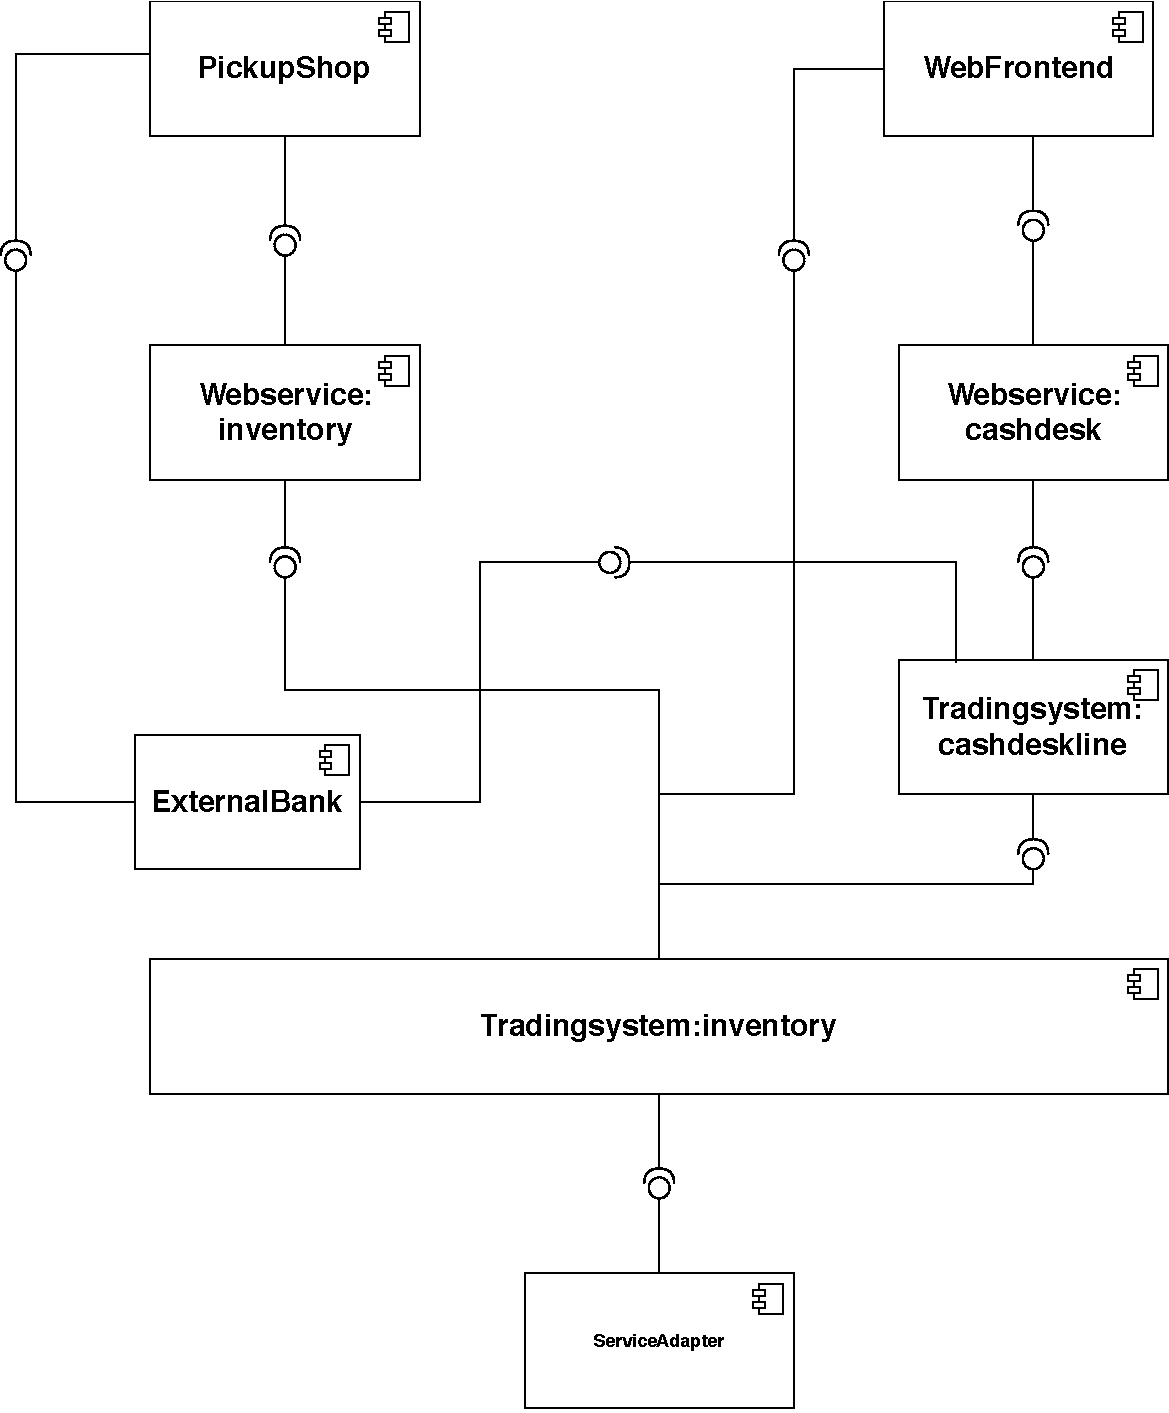
\includegraphics[scale=.7]{logos/ArchPickupShop.pdf}
\caption{The figure shows a simplified overview over the hybrid cloud based variant}
\label{fig:genArch}
\end{figure}
%evolutionary scenarios
%platform migration
\subsection{Platform migration}
The first evolutionary scenario is platform migration. This is done to reduce the costs. The CoCoME system is moved to a cloud environment for easier scalability. If, for example, the pickup shop is heavily used due to a large advertisement campaign, additional resources in order to compensate for bottlenecks, can easily be purchased.\\ 
\subsection{Addition of a Pickup shop}
\label{subsec:PS}
The next evolutionary scenario is the addition of a Pickup shop to CoCoME. The Pickup shop offers a second Point-of-Sale for CoCoME to concurrent with web shops like Amazon. Customer may order products online and pick them up in their chosen store. Therefore an account in the CoCoME system is required. With the Pick up shop, CoCoME changes from a closed to an open system. As shown in \autoref{fig:genArch}, the \textit{PickupShop} bypasses the  \textit{Tradingssystem:cashdeskline} and directly accesses the\textit{Tradingssystem:inventory}. The payment process is carried out in the \textit{PickupShop} component.

\subsection{Database migration}
In this evolutionary scenario the database is migrated to a cloud service. Due to the fact, that the PickupShop and the stores both operate on the inventory, a higher amount of database request is expected. In order to avoid possible shortcomings in the performance, the database was moved to a cloud environment. This allows to easily purchase additional bandwidth or space to solve upcoming scalability issues. With the migration of the database a new issue arise. It may happen, for example, that data from enterprises that are located in the European Union (EU) are stored outside the EU, which does not comply with the current law.
\subsection{Service adapter}
%TODO nochmal genauer, Unterschied zu Webservice
Since CoCoME was always in development, CoCoME currently consists of a relatively large code base. Since this does not have to be understood by every single developer to work with CoCoME, a service adapter has been added. The service adapter allows CoCoME to dynamically add functionality.
\paragraph{Reasons for CoCoME to apply our procedure on}
The decision to use CoCoME as the system for applying the method was based on many reasons. The first is that CoCoME has already been modeled as a component-based system. Another reason is that CoCoME is described in detail in \cite{CoCoMETechReport} and the CoCoME book \cite{CoCoMEBook}. 
On the other hand, CoCoME is more of a minimal solution to what is actually planned to achieve with CoCoME. One can say, CoCoME is rather a proof of concept than a fully functional system.
%TODO  Nur der PickupShop betrachtet
\section{Application of the method}
\label{apllMethod}
After an short overview over CoCoME in the previous section, we are starting with the procedure for the creation of a case study. The presented paper from Runeson and H\"ost \cite{CaseStudySoftware}, which is could be seen as a fundamental source for the creation of case studies, states that one should use more than one source of information for the investigated case. We used as our main source of information the CoCoME tech report \cite{CoCoMETechReport} and the CoCoMe book \cite{CoCoMEBook}, were the system is described in detail. Further we used the code of the implementation.
%github referenzieren
. If there are differences between documentation and code, the definitions from the documentation applies. We favour the documentation over the code because CoCoME is still in development. The documentation represents a stable version of CoCoME. In the implementation it may possible that at the moment new features are tested that are later quashed.\\  We do not apply the process to the entire CoCoME system, but concentrate on only part of the system. The selected part of CoCoME is the PickupShop (\autoref{PS}).
\subsection{P1: Investigation of the current state of CoCoME}
%done
In this first step we take a first look at CoCoME. We are looking for two main aspects here. First, if the system is extendable. Secondly, how wide spread the system model already is defined. The CoCoME include a book \cite{CoCoMEBook}, a tech report \cite{CoCoMETechReport} and an implementation. In the documentation CoCoME various system models for CoCoME are available and CoCoME is modeled as an component-based system and therefore extendable. So we decided that the system is in viable state.%TODO githubs referenzieren
%TODO hier noch genauer werden \\
In the case of CoCoME, a tech report \cite{CoCoMETechReport}, a book \cite{CoCoMEBook} and an implementation is available. For the fact, that CoCoME is modelled as a component-based system, the system is also  extendable.
\subsection{P2: Extract the necessary system parts for the requirements}
\label{reqCoCoME}
In the next step, we identify the necessary system parts in CoCoME for the six requirements listed in \autoref{req_over_cocome}. In the following, for each requirement the related system parts are extracted. 
\begin{table}
\begin{tabular}{|c|c|}
\hline 
\multicolumn{2}{|c|}{Requirements} \\ 
\hline 
R1 & Component based system \\ 
\hline 
R2 & Use cases \\ 
\hline 
R3 & Security relevant data \\ 
\hline 
R4 & User roles \\ 
\hline 
R5 & Access rights \\ 
\hline 
R6 & Type of data processing in components \\ 
\hline 
\end{tabular} 
\caption{Overview for the requirements for a case study}
\label{req_over_cocome}
\end{table}

\subsubsection{R1: Component based system}
This requirement is met because a component-based system model is defined in the CoCoME tech report\cite{CoCoMETechReport}.
\subsubsection{R2: Existence of use cases}
\label{req_uc}
The CoCoME documentation defines thirteen use cases, so this requirement is also met. The use cases are defined in detail either in the CoCoME book \cite{CoCoMEBook} in the CoCoME tech report \cite{CoCoMETechReport}. 
\subsubsection{R3: Security relevant data}
\label{req_data}
%Sollte fertig ein !!!
Since the amount of data is relatively large in the investigated excerpt of CoCoME, we have grouped the data into different equivalence classes. The data type in each class has the same security level. Composite data types inherit the security levels from most restrictive class. We defined four classes: \textbf{customer data}, \textbf{account data}, \textbf{product\&sales data} and \textbf{system data}. 
\begin{itemize}
\item Customer data\\ This class describes all data types that are provided by the customer role. This includes names, addresses and credit card details, to name the most important ones. %Since it is personal data of an entity , we classified it as \textbf{security relevant data}.
\item Product\&Sales data \\ All the data that is related to the products and the sales process. Examples for data types are price of a product, quantity of a product, date of shipping etc. %Data in this class may become security relevant if it enables traceability to security relevant data. For this fact product and sales related data is not defined strictly security relevant. Nonetheless, access to this data can cause damage to an enterprise. 
\item Account data \\ Account related data refers to the introduced accounts with he addition of the PickupShop. It is needed that each role is registered with an account in the system. The account data type holds the \textit{username} and the credentials for an account. %We classified this data as \textbf{security relevant}, because access to account data allows to log in as the role.
\item System data \\ In this class mainly summarizes the created queries for access to the underlying database. %Access to the issued queries allows to cause damage in a lot of different ways. It is possible to, for example, alter the database, read user informations, etc. Therefore this data is classified \textbf{security relevant}.
\end{itemize}
The security relevance for each class is defined according to Breier's approach \cite{assetValue}. The approach is based on the possible damage the loss of an asset could cause. So for each asset the level of damage a loss of the asset could cause is defined. Further, for each asset the dependencies to other assets is defined. Based on this, it is possible to calculate the value of an asset. This approach is not one-to-one applicable to our case, but we can use the basic idea. We evaluated for each data class the possible impact a leak of data from this class may have in CoCoME. Keep in mind that the primary goal is to protect persons that are using CoCoME. Therefore, the customer data is the most relevant and defined as \textbf{security relevant}.\\ The account data allows to log in as the specific role, which may lead to leaks of the customer's personal data. So the account data is also \textbf{security relevant}. The system data mostly consists of queries. If one may gain access to the query, it is to alter the database. So this data is especially \textbf{security relevant}, because access to it may cause damage to the customer and the enterprise in the same scale.\\ At last, the product\&sales data is not considered strictly security relevant, because in the sales process the payment process as we identify it is part of the customer data. This data becomes relevant in composite data types or if it allows traceability to customer data. Nonetheless, leak in this class may cause heavy damages to the respective enterprise, which is not in the scope of the thesis.
\subsubsection{R4: roles}
\label{req_roles}
CoCoME defines six different roles. Five are defined in the CoCoME tech report \cite{CoCoMETechReport}. These are the \textit{Customer}, the \textit{Cashier}, the \textit{StoreManager}, the \textit{Enterprise manager}, and the \textit{Stockmanager}. The last role, the \textit{Admin},  appears in the code. In the documentation, there is no separate description of the roles. All the responsibilities are derived from the use cases described in the documentation and/or the implementation. The key information we are looking for, are the tasks that a role performs in the context of CoCoME and which data is provided/required by the role. 
\begin{itemize}
\item  After analyzing the implementation, the \textit{Customer} role is the role of all the customers of an enterprise, be they private customers or business customers. The role buys products, either in the stores or in the Pickup shop. The data provided by the customer role are the customer related data, It requires product related data to, for example, decide which products to buy.
\item For the \textit{Cashier} role, we rely on the defined use cases in CoCoME tech report. As shown, the role takes over the sale of products and therefore requires product \& sales data. The role provides product and sales-related data like the data that is generated when orders are placed.
\item For the \textit{StoreManager} role, we relied on the use cases. The \textit{StoreManager} handles the tasks of a single store. The role provides and requires product\& sales related data.
\item After an analysis of the use cases, we are not sure what the concrete tasks are for the \textit{EnterpriseManager} and the data requires requires or provide. There are only two uses cases that involves the \textit{EnterpriseManager}, therefore a clear definition is not possible. Unfortunately, the code does not contain any further information. From the name it can be derived that the role is in charge of a  whole enterprise. 
\item After analyzing the use cases, it is clear that the \textit{StockManger} handles the stock of a single store. Therefore the role requires product\&sales related data and provides the same type in the system.
\item After analyzing the code we found a sixth role, the \textit{Admin} role. This role is not mentioned in the use cases. From the name alone, we assume that this role keep a watch on the system. But use cases are missing and the implementation do not allow to define neither the tasks nor the provided/required data.
%TODO revisit admin in the system extension
\end{itemize}
Since the hybrid cloud based variant is examined by us, all roles provide account data, because each role, in the hybrid cloud-based variant, needs an account in CoCoME to access the system. 
\subsubsection{R5: access rights}
To define the access rights, we use the finer grained, high level from proposed by Evered and Bögeholz \cite{CaseStudyAndAccessrigths} in contrast to the well known read/write semantics for access control. %We tried not to rely on a read/write semantic to allow a more detailed description of the access rights.
Therefore, as described in \autoref{ch:method}, it is defined for the data present in a component how which role can access it. We defined four different privilege level for the access to data, presented in the following enumeration. We used the  elements from the previous requirements R2 (\nameref{req_uc}), R3 (\nameref{req_data}) and R4 (\nameref{req_roles}) to derive the access rights for CoCoME. The access to data decreases with the ascending numbers.
\begin{enumerate}
\item \textbf{FullAccess}\\ This access rights defines that the associated role has access to all data types for the respective class in the component.
\item \textbf{AccessToUsedData}\\ This access right defines that the role has accessed to it used data types for the respective class in the component. Used data in this context means the data types that are required by the role to perform its defined tasks.
\item \textbf{AccessToOwnedData}\\ This access right defines that the associated role has access to its , for example, own account data or customer data. This access rights ensures that roles may access data that is provided by it but not necessarily needed for their tasks.
\item \textbf{Default} This access right forbids the complete access to all data in a class for this role and component.
\end{enumerate}

\begin{figure}
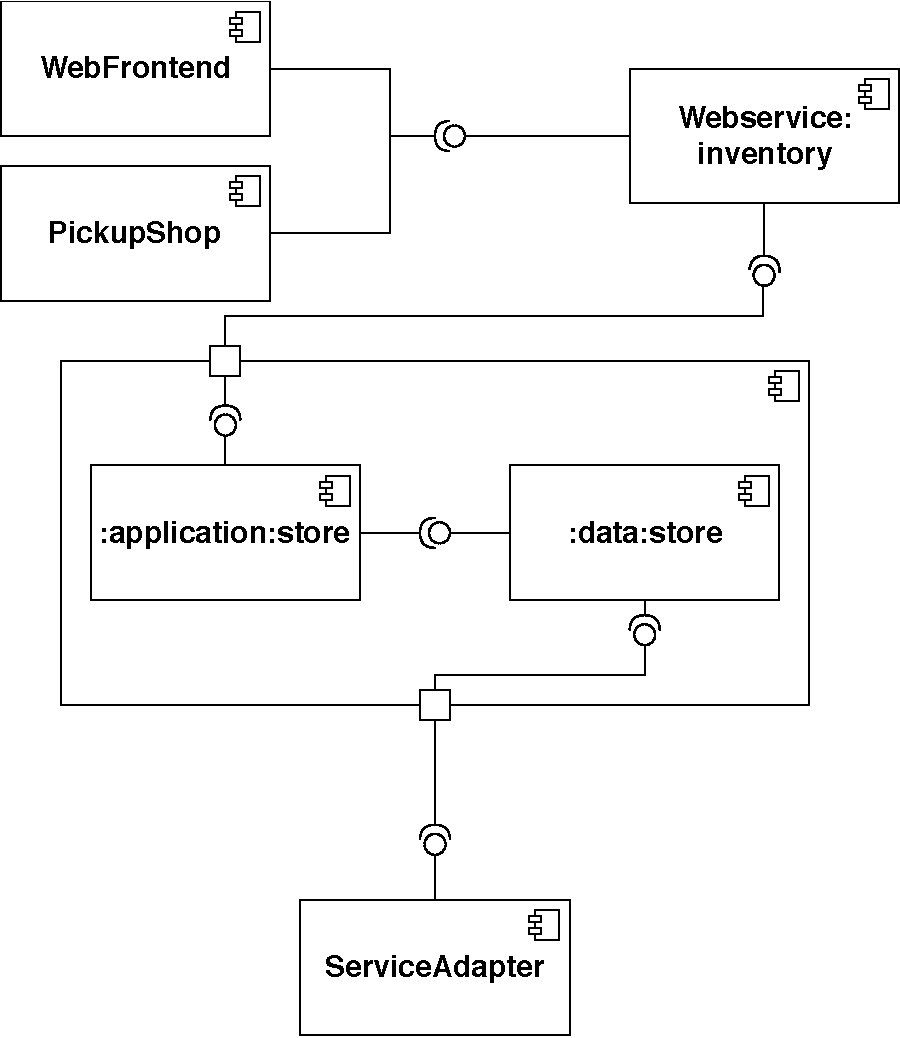
\includegraphics[scale=.8]{logos/ExcerptRelComps.pdf}
\caption{The figure shows an simplified overview of the CoCoME. The Webservice component is omitted.}
\label{CoCoME_simplified}
\end{figure}
%TODO access rights matrix für CoCoME aufstellen
Another part of this requirement is the identification of the present data types in each component. After analyzing the code and the CoCoME tech report, we identified data for each class of data in each component. Also we identified that no role except the \textit{customer} may access the \textit{PickupShop} component. A  reduced system model is displayed in \autoref{CoCoME_simplified}. As already mentioned in \autoref{sec:cocome_overview}, it is only possible for individual users to interact with CoCoME via the components \textit{Webfrontend} and \textit{PickupShop}. No role except the admin has direct access to the \textit{Tradingsystem:inventory} component in which the data is processed. Therefore, all access rights to data are cascaded for the individual roles (except the admin). This ensures that it is always visible which role receives which data or has provided which data. \\
For the fact that the ACM in \autoref{ACMConcept} is rather large and complex, we only point out the most important points. We omitted the \textit{Webservice} component, as it only transmits data between the user interface and the \textit{Tradingsystem:inventory} and therefore has no effect on the data. As stated before, only the \textit{customer} may access the \textit{PickupShop}, therefore no other role may access the data in this component. For the \textit{Admin} it is not clear if the role may access data. Also, the \textit{Admin} it the only role that may access \textit{system} data. The \textit{StockManager} has access to customer data due to the use cases. In 
\begin{landscape}
\begin{table}
\begin{tabular}{|c|c|c|c|c|}
\hline 
ACM & Webfrontend & PickupShop & TS:inventory & TS:inventory \\ 
& & & data & application \\
\hline 

customer 
& \begin{tabular}{c|c}
customer data & 3 \\
account data & 3 \\
p\&s data & 3 \\
system data & 4 \\
\end{tabular}
&
\begin{tabular}{c|c}
customer data & 3 \\
account data & 3 \\
p\&s data & 3 \\
system data & 4 \\
\end{tabular} 
&
%TS:inv:data
 \begin{tabular}{c|c}
customer data & 3 \\
account data & 3 \\
p\&s data & 3 \\
system data & 4 \\
\end{tabular}
& 
%Ts:inv:app
\begin{tabular}{c|c}
customer data & 3 \\
account data & 3 \\
p\&s data & 3 \\
system data & 4 \\
\end{tabular}
 \\ 
\hline 
cashier 
& 
%WF
 \begin{tabular}{c|c}
customer data & 3 \\
account data & 3 \\
p\&s data & 2 \\
system data & 4 \\
\end{tabular}
&
%PS
 \begin{tabular}{c|c}
customer data & 4 \\
account data & 4 \\
p\&s data & 4 \\
system data & 4 \\
\end{tabular}
&
%TS:cdl
 \begin{tabular}{c|c}
customer data & 3 \\
account data & 3 \\
p\&s data & 2 \\
system data & 4 \\
\end{tabular}
&
%TS:inv
 \begin{tabular}{c|c}
customer data & 3 \\
account data & 3 \\
p\&s data & 2 \\
system data & 4 \\
\end{tabular} 
 \\ 
\hline 
StockManager 
&
%WF
 \begin{tabular}{c|c}
customer data & 2 \\
account data & 3 \\
p\&s data & 2 \\
system data & 4 \\
\end{tabular}
&
%PS
 \begin{tabular}{c|c}
customer data & 4 \\
account data & 4 \\
p\&s data & 4 \\
system data & 4 \\
\end{tabular}
&
%TS:cdl
 \begin{tabular}{c|c}
customer data & 4 \\
account data & 4 \\
p\&s data & 4 \\
system data & 4 \\
\end{tabular}
&
%TS:inv
 \begin{tabular}{c|c}
customer data & 2 \\
account data & 3 \\
p\&s data & 2 \\
system data & 4 \\
\end{tabular}

  \\ 
\hline 
EnterpriseManager & 
 
%WF
 \begin{tabular}{c|c}
customer data & 2 \\
account data & 2 \\
p\&s data & 2 \\
system data & 2 \\
\end{tabular}
&
%PS
 \begin{tabular}{c|c}
customer data & 2 \\
account data & 2 \\
p\&s data & 2 \\
system data & 2 \\
\end{tabular}
&
%TS:cdl
 \begin{tabular}{c|c}
customer data & 2 \\
account data & 2 \\
p\&s data & 2 \\
system data & 2 \\
\end{tabular}
&
%TS:inv
 \begin{tabular}{c|c}
customer data & 2 \\
account data & 2 \\
p\&s data & 2 \\
system data & 2 \\
\end{tabular}
 \\ 
\hline 
StoreManager & 
 
%WF
 \begin{tabular}{c|c}
customer data & 2 \\
account data & 3 \\
p\&s data & 2 \\
system data & 4 \\
\end{tabular}
&
%PS
 \begin{tabular}{c|c}
customer data & 4 \\
account data & 4 \\
p\&s data & 4 \\
system data & 4 \\
\end{tabular}
&
%TS:cdl
 \begin{tabular}{c|c}
customer data & 2 \\
account data & 3 \\
p\&s data & 2 \\
system data & 4 \\
\end{tabular}
&
%TS:inv
 \begin{tabular}{c|c}
customer data & 2 \\
account data & 3 \\
p\&s data & 2 \\
system data & 4 \\
\end{tabular}
 \\ 
\hline 
Admin 
%WF
& \begin{tabular}{c|c}
customer data & ? \\
account data & ? \\
p\&s data & ? \\
system data & 1 \\
\end{tabular}
&
%PS
\begin{tabular}{c|c}
customer data & ? \\
account data & ? \\
p\&s data & ? \\
system data & 1 \\
\end{tabular} 
&
%TS:inv:app
 \begin{tabular}{c|c}
customer data & 1 \\
account data & 1 \\
p\&s data & 1 \\
system data & 1 \\
\end{tabular}
& 
%Ts:inv
\begin{tabular}{c|c}
customer data & 1 \\
account data & 1 \\
p\&s data & 1 \\
system data & 1 \\
\end{tabular}
 \\ 
\hline 
\end{tabular} 
\caption{The ACM of CoCoME. The legend for the ACM is: 1 is the access right \textit{FullAccess}, 2 is the access right \textit{AccessToUsedData}, 3 is the access right \textit{AccessToOwnedData}, 4 is the access right \textit{Default}. The abbreviation \textit{p\&s data} stands for product\&sales  data.}
\end{table}
\label{ACMConcept}
\end{landscape}

\subsubsection{R6: Type of data processing in components}
\label{relevantpartsCoCoME}
%TODO hier ist meine achilles ferse !!!!!
The last requirement defines the different types how data is processed in CoCoME. For each component, it is defined how the data from the different data classes is processed in this specific component. To identify the different types of processing we analyzed the code and the use cases. All in all, we defined four different classes how data is processed in CoCoME. Each class may consists of various operations.
\begin{itemize}
\item relational algebra \\ This type describes the operations of relational algebra on a database or similar construct. For example, if all elements of a list that have a particular ID are selected from this list.
\item transmission of data \\ This type describes the transmission of data between components.
\item alternation of data \\ This type includes the most operations. It describes each operation that changes the data class. Good examples are the creation of lists or the merging two or more data classes into one.
\item I/O related processing \\  This type describes the user interaction with CoCoME. 
\end{itemize}
After the different classes of data processing are identified, we analyzed how which data is processed in each component. The respective type(s) of data processing are assigned to the respective components. The result is shown in \autoref{typeMatrix}. \\
%Erklärung warum wie zugeordnet wurde.
\textit{System} data is not available in any other component other than \textit{Tradingssystem:inventory:data}, because in this component queries are created. The \textit{Webservice} component only transmit data to other components. The \textit{PickupShop} and \textit{Webfrontend} transmits the \textit{customer} and \textit{account} data. In these to components the user interfaces are located and customer, for example, fill their shopping cart, therefore \textit{products\&sales} data is processed with the \textit{I/O} processing.

%Then we have assigned one or more types for each component and each role. We omitted the Webservice component because it only delegates the data to other components and has no effect on the result. The result is shown in \autoref{typeMatrix}. In the matrix for each data class it is defined how which this data class can be processed in the components.To give simple example, in the \textit{Webfrontend} the customer data can only be transmitted to other components. In the \textit{Tradingsystem:inventory:application}, the same data may also be changed to another data class. As shown, we divided the Trandingsystem:inventory component. This was done because the sub-components have different type of processing. 

\begin{table}
\begin{tabular}{|c|c|c|c|c|}
\hline 
Types of  & Customer & Account & Product\&sales & System  \\ 
data processing  & data & data & data & data \\
\hline 
Webfrontend &  transmit & transmit & I/O-processing & non-existent \\ 
& & &  transmit & \\
\hline 
PickupShop &  transmit & transmit & I/O-processing, & non-existent \\ 
& & & transmit & \\
\hline 
Tradingsystem:& change & alter & alter & non-existent \\ 
inventory: & transmit& transmit & & \\
application & & & & \\
\hline 
Tradingsystem: & relational algebra& relational algebra& relational algebra& alter \\
inventory:data & operations & operations & operations & \\ 
\hline
Webservice & transmit & transmit & transmit & transmit \\
\hline 
\end{tabular} 
\caption{Overview of the different types of data processing in the components. For each component, it is defined how which data class can be processed.}
\label{typeMatrix}
\end{table}
\subsection{P3: Check the fulfillment of the requirements}
\label{shortcommingsCoCoME}
Once the system parts for each requirement have been identified, defined or derived, a brief check is made to ensure that each requirement has been met. For each requirement it is checked whether the individual system elements are complete. It is possible that some definitions are vague or missing. Vague means that there is room for interpretation or that different definitions contradict each other. \\ In the following, we analyzed the fulfillment for each individual requirement. 
\subsubsection{R1: component-based systems}
This requirement is fulfilled, a very detailed component for CoCoME is provided \cite{CoCoMETechReport}.
\subsubsection{R2: use cases}
A detailed use case diagram with a brief description of each use case is provided in the CoCoME tech report \cite{CoCoMETechReport}. All in all, 13 use cases are defined, which cover the main aspects of CoCoME.
\subsubsection{R3: security relevant data}
% Report nicht richtig definiert, Verbindung zwischen custome rund seinen Produkten, 
In the definition of the data, a lot of data is already defined by the implementation. Nonetheless, some data mentioned in the use cases is missing. We identified in the investigated excerpt two missing data types. First, there is no connection defined between the customer and the purchased products. Secondly, the \textit{Report} data type mentioned in the use cases is also not defined.
\subsubsection{R4: definition of roles}
For some roles the actual tasks are not clear because some use cases contradict each other. Further, for the \textit{EnterpriseManager} there are too few use cases to clearly define the tasks. For the \textit{Admin} role use cases are completely missing, because this role is only present in the code.
\subsubsection{R5: definition of access rights}
In the case of the access rights we cannot say in general if they are fulfilled, because the access rights are derived from the previous requirements R1-R4. If there are changes in R1-R4, the defined access rights have to be reviewed and if necessary updated. Nonetheless, in the case \textit{Admin} the tasks for this role are not clear, therefore it was not possible to derive access rights in some cases. 
\subsubsection{R6: types of data processing in the components}
This requirement is adjacent to R5: definiton of the access rights. The different types of data processing are derived from the previous requirements R1-R4. If there are changes in R1-R4, the different types of data processing have to be reviewed and if necessary updated.
\subsection{P4: Define system extensions}
In the next step, we define system extensions for CoCoME to fix all shortcomings for the requirements. In the previous step all shortcomings were summarized. In the following, we give an overview how CoCoME was extended to meet all requirements.

\paragraph{R1: component-based system}
Here, no extensions was needed, because this requirement is met.
\paragraph{R2: definition of use cases}
Also, no need to define an extensions. This requirement is also met.
\paragraph{R3: security relevant data}
As identified previously in \autoref{shortcommingsCoCoME}, two data types are missing. First, there are no connection defined between a customer and its purchased products. Secondly, the \textit{Report} data type is only mentioned but is not defined.
\begin{itemize}
\item Connection between customer and purchased products\\ We defined that the connection is realized by adding a list of all orders to the customer object. Each order in CoCoME includes the involved products and other information like the total price. 
%TODO WARUM -> overhead, cust obj is eh schon geschützt, .... GUT muss sie sein
\item Report data type\\ We have defined this data type as a string that can be read by humans.
\end{itemize}
\paragraph{R4: definition of roles}
For the fourth requirement, two roles need a clearer definition: the \textit{EnterpriseManager} and the \textit{Admin}.In the case of the \textit{EnterpriseManager} there are too few use cases are defined to clearly derive tasks for this role. In the case of the \textit{Admin} there are no use cases defined. because this role only exists in the code. 
\begin{itemize}
\item EnterpriseManager \\
Due to the fact, that only one use case is defined for the \textit{EnterpriseManager}, the actual tasks for this role are not clear. So determined that the role is in charge of a whole enterprise. For the fact that a \textit{StockManager} manages the stock for each store, we defined the \textit{EnterpriseManager} works on a larger scale. The role monitors the workflows within an enterprise and calculates forecasts for, for example, the CPU capacity required. Therefore, the \textit{EnterpriseManager} provides product\&sales data and requires customer data, account data and product\&sales data. For the customer and account data, the role only requires meta data, like the number of registered accounts and therefore no explicit data. 
\item Admin \\
The \textit{Admin} has no use cases associated, so we relied on the implementation. In the implementation, the role has access to all data, so we defined the \textit{Admin} to be the master role in the system, that has access to all data. With access to all data any small or big problems may be reviewed and fixed. Therefore the role provides and requires all data types.
\end{itemize}
\paragraph{R5: definition of access rights}
Since the previous requirements are  fulfilled with the defined system extensions, in this step the ACM is reviewed and updated. The updated ACM is shown in \autoref{ACM_updated}. The entries that have changed since the old version are shown in bold. As before, the \textit{Webservice} component is omitted.

\begin{landscape}
\begin{table}
\begin{tabular}{|c|c|c|c|c|}
\hline 
ACM & Webfrontend & PickupShop & TS:inventory: & TS:inventory: \\ 
& & & data & application \\
\hline 
customer 
%WF
& \begin{tabular}{c|c}
customer data & 3 \\
account data & 3 \\
p\&s data & 3 \\
system data & 4 \\
\end{tabular}
&
%PS
\begin{tabular}{c|c}
customer data & 3 \\
account data & 3 \\
p\&s data & 3 \\
system data & 4 \\
\end{tabular} 
&
%TS:cdl
 \begin{tabular}{c|c}
customer data & 3 \\
account data & 3 \\
p\&s data & 3 \\
system data & 4 \\
\end{tabular}
& 
%Ts:inv
\begin{tabular}{c|c}
customer data & 3 \\
account data & 3 \\
p\&s data & 3 \\
system data & 4 \\
\end{tabular}
 \\ 
\hline 
cashier 
& 
%WF
 \begin{tabular}{c|c}
customer data & 3 \\
account data & 3 \\
p\&s data & 2 \\
system data & 4 \\
\end{tabular}
&
%PS
 \begin{tabular}{c|c}
customer data & 4 \\
account data & 4 \\
p\&s data & 4 \\
system data & 4 \\
\end{tabular}
&
%TS:cdl
 \begin{tabular}{c|c}
customer data & 3\\
account data & 3\\
p\&s data & 2\\
system data & 4\\
\end{tabular}
&
%TS:inv
 \begin{tabular}{c|c}
customer data & 3\\
account data & 3\\
p\&s data & 2\\
system data & 4\\
\end{tabular} 
 \\ 
\hline 
StockManager 
&
%WF
 \begin{tabular}{c|c}
\textbf{customer data} & \textbf{4}\\
account data & 3\\
p\&s data & 2\\
system data & 4\\
\end{tabular}
&
%PS
 \begin{tabular}{c|c}
customer data & 4\\
account data & 4\\
p\&s data & 4\\
system data & 4\\
\end{tabular}
&
%TS:cdl
 \begin{tabular}{c|c}
customer data & 4 \\
account data & 4 \\
p\&s data & 4 \\
system data & 4 \\
\end{tabular}
&
%TS:inv
 \begin{tabular}{c|c}
\textbf{customer data} & \textbf{4} \\
account data & 3 \\
p\&s data & 2 \\
system data & 4 \\
\end{tabular}

  \\ 
\hline 
EnterpriseManager & 
 
%WF
 \begin{tabular}{c|c}
\textbf{customer data} & \textbf{1} \\
\textbf{account data} & \textbf{1} \\
\textbf{p\&s data} & \textbf{1} \\
\textbf{system data} & \textbf{4} \\
\end{tabular}
&
%PS
\begin{tabular}{c|c}
\textbf{customer data} & \textbf{1} \\
\textbf{account data} & \textbf{1} \\
\textbf{p\&s data} & \textbf{1} \\
\textbf{system data} & \textbf{4} \\
\end{tabular}
&
%TS:cdl
\begin{tabular}{c|c}
\textbf{customer data} & \textbf{1} \\
\textbf{account data} & \textbf{1} \\
\textbf{p\&s data} & \textbf{1} \\
\textbf{system data} & \textbf{4} \\
\end{tabular}
&
%TS:inv
\begin{tabular}{c|c}
\textbf{customer data} & \textbf{1} \\
\textbf{account data} & \textbf{1} \\
\textbf{p\&s data} & \textbf{1} \\
\textbf{system data} & \textbf{4} \\
\end{tabular}
 \\ 
\hline 
StoreManager & 
 
%WF
 \begin{tabular}{c|c}
customer data & 2 \\
account data & 3 \\
p\&s data & 2 \\
system data & 4 \\
\end{tabular}
&
%PS
 \begin{tabular}{c|c}
customer data & 4 \\
account data & 4 \\
p\&s data & 4 \\
system data & 4 \\
\end{tabular}
&
%TS:inv:data
 \begin{tabular}{c|c}
customer data & 2 \\
account data & 3 \\
p\&s data & 2 \\
system data & 4 \\
\end{tabular}
&
%TS:inv:app
 \begin{tabular}{c|c}
customer data & 2 \\
account data & 3 \\
p\&s data & 2 \\
system data & 4 \\
\end{tabular}
 \\ 
\hline 
admin & 
%WF
 \begin{tabular}{c|c}
customer data & \textbf{1} \\
account data & \textbf{1} \\
p\&s data & \textbf{1} \\
system data & \textbf{1} \\
\end{tabular}
&
%PS
 \begin{tabular}{c|c}
customer data & \textbf{1} \\
account data & \textbf{1} \\
p\&s data & \textbf{1} \\
system data & \textbf{1} \\
\end{tabular}
&
%TS:inv:data
 \begin{tabular}{c|c}
customer data & \textbf{1} \\
account data & \textbf{1} \\
p\&s data & \textbf{1} \\
system data & \textbf{1} \\
\end{tabular}
&
%TS:inv:app
 \begin{tabular}{c|c}
customer data & \textbf{1} \\
account data & \textbf{1} \\
p\&s data & \textbf{1} \\
system data & \textbf{1} \\
\end{tabular}
 \\ 
\hline 
\end{tabular} 
\caption{The updated Version of the ACM for CoCoME after the shortcomings are fixed. The legend for the ACM is: 1 is the access right \textit{FullAccess}, 2 is the access right \textit{AccessToUsedData}, 3 is the access right \textit{AccessToOwnedData}, 4 is the access right \textit{NoAccess}. The bold entries changed since the old version.}
\label{ACM_updated}
\end{table}
\end{landscape}
\paragraph{R6: types of data processing in the components}
%TODO eventuell noch ein bisschen besser schreiben !!!!
The different types of data processing are also derived from the requirements R1-R4. After reviewing the different types of data processing that were defined, there are no need to extend anything. 
\subsection{P5: Evaluation of the defined access rights}
After all system extensions are done, in this step  the defined access rights are evaluated. The evaluation follows a GQM-plan %TODO ref auf foundations
The GQM-plan for the evaluation of the access rights is shown in
\begin{figure}

\caption{GQM-plan for the evaluation of the defined access rights. The evaluation focus on the highlighted parts.}
\label{evalAR}
\end{figure}
 %TODO ref figure
\subsubsection{Goal: Evaluation of the case study}
The goal is to evaluate the case study. A shown in \autoref{evalAR} the evaluation of the case study is split into two parts. In this we will only focus on the highlighted plan, the evaluation of the access rights.
\subsubsection{Question: Are the access rights well defined ?}
Well defined access rights means in this context that the defined access rights meet the criteria defined by Evered and Bögeholz\cite{CaseStudyAndAccessrigths}.The two authors defined seven different criteria. In order to ensure well defined access rights, the seven criteria should be met. The seven criteria are : Concise, clear, aspect-oriented, fundamental, positive, need-to-know and efficient. We categorized the criteria into three classes: specification, comprehensibility and implementation. The division of the individual criterion into categories is shown in \autoref{fig:Class_ARC}.
%TODO in paragraphen 
\begin{table}
\centering
\begin{tabular}{|c|c|}
\hline 
\multicolumn{2}{|c|}{Access rights} \\ 
\hline 
Specification & Aspect-oriented  \\ 
\hline 
 & Positive  \\ 
\hline 
 & Need-to-know \\ 
\hline 
Comprehensibility & Clear \\ 
\hline 
 & Concise  \\ 
\hline 
Implementation & Fundamental \\ 
\hline 
 & Efficient \\ 
\hline 
\end{tabular} 
\caption{Classification of the criteria for good access rights.}
\label{fig:Class_ARC}
\end{table}
The criteria in the class \textit{Specification} evaluate the properties of the defined access and the general access levels that that well defined access rights cover.\\
The criteria in the class\textit{Comprehensibility} evaluates the complexity of the notation.\\
The criteria in the class \textit{Implementation} evaluate the embedding of the access rights in the implementation.\\
It was possible to only evaluate three of the seven criteria due to various reasons. \textit{Comprehensibility} criteria ware not possible due to time constraint. The criteria in this class are checked by conducting a survey. This was not possible in the time frame of this thesis. For the \textit{Implementation} criteria an integration of the access rights into the implementation of CoCoME is needed. This implementation is missing, so it was also not possible to check this class.\\
The remaining criteria \textit{Aspect-oriented}, \textit{Positive} and \textit{Need-to-know} located in the \textit{Specification} class. \\
\textit{Aspect-oriented} deswcribes, that the implementation and the access rights are sperate stored and define. This alloows that the implementation and the access rights can be used in different contexts. Further, both are easier to understand , if they are separated.  \\
\textit{Positive} describes, that the access to data have to explicitly given to the entities. The default level of access is \textit{no access}. This avoid that access is implicitly granted.\\
\textit{Need-to-know} describes, that well defined access rights only allow access to the absolute minimum of data that are used by the entities. \\

\subsubsection{Metric Number of satisfied criteria}
The evaluation is done in a checklist manner. For each criterion the defined access rights are evaluated whether they fulfill this criterion. The results of the metric are summarized in \autoref{AR_EVAL_SUM}.
\begin{table}
\begin{tabular}{|c|c|c|}
\hline 
\multicolumn{2}{|c|}{Access rights} & fulfilled? \\ 
\hline 
Specification & Aspect-oriented & \cmark
 \\ 
\hline 
 & Positive & \cmark 
 \\ 
\hline 
 & Need-to-know & \cmark 
 \\ 
\hline 
Comprehensibility & Clear & ? \\ 
\hline 
 & Concise & ? \\ 
\hline 
Implementation & Fundamental & n/a \\ 
\hline 
 & Efficient & n/a \\ 
\hline 
\end{tabular} 
\caption{Summary for the evaluation of the defined access rights.} 
\label{AR_EVAL_SUM}
\end{table} 
\paragraph{Aspect-oriented}
%Beschreibung des Kriteriums danach 
The access rights are stored separately from the code and even from the defined data flows. The access rights are changeable in the context of the case study. This allows that a scenario may be evaluated in different security contexts. So this criterion is met.
\paragraph{Positive}
The created case study achieves this criterion. First, granular access control rights have been defined. The access rights are differentiated in four different levels and each level represents fine grained access. We also defined a default value, which represents \textit{no access} to data. 
\paragraph{Need-to-know}
This criterion is achieved by the created case study. We split the data in four classes. For each component it is defined which role has access to which data. With this we can model, for example, that a role may access data in component A but not in component B. Further the differentiation in four levels allows, for example, to explicitly distinguish between access to data provided by that role and access to data that is not provided, but needed for the role's tasks. so this criteria is also met 
\paragraph{Concise and clear}
Due to the time frame of the thesis, we could not make a qualified statement if these criteria are met.
\paragraph{Fundamental and Efficient}
Since access control is not yet part of the implementation, it was not possible to check it at all.
\subsection{M1: Store the current state in a milestone}
Before the current system state is saved in the milestone, one have to decide if the access rights are well defined. After that the milestone is created. The milestone stores for each requirement the necessary model elements.
\paragraph{Quality of access rights}
The defined access rights achieved all criteria that we were able to check. So we summarize that the defined access rights are for the moment well defined. So the procedure moves to the next step and the current system state is stored in a milestone.
\paragraph{Milestone}
For each requirement the associated system elements are stored.
\begin{itemize}
\item R1: The system model\\ In this particular milestone, the system model from the CoCoME tech report \cite{CoCoMETechReport} is stored.
\item R2: Use case diagram, definition for each use case.\\  In this particular milestone, the use case digram from the CoCoME tech report \cite{CoCoMETechReport} is stored.
\item R3: The data types and the examination, which data is security relevant. \\ the four data classes ans the respective description of them are stored.
\item R4: The different user roles\\ The description of the tasks and the provided/required data for each role are stored. The \textit{Admin} role is explicitly stored, because this role is not mentioned in the stored use case diagram.
\item R5: The created ACM \autoref{ACM_updated}.
\item R6: The created OpM \autoref{typeMatrix}.
\end{itemize}
\chapter{Case study system}
\label{ch:casestudysystem}
%Was wir dheir geschehen und kurz einleiten
After we reached the milestone in the last chapter, we are going to define scenarios, evaluating the defined scenarios and concluding the procedure in this one.\\
A scenario is a actual characteristics from, for example, a use case. But scenarios in general describe a actual interaction by one or more users with the system. This scenarios are later converted in data flows that are added to the system model. The scenario created by using the ACM \autoref{ACM_updated} and the OpM \autoref{typeMatrix}. We defined two scenarios for CoCoME.\\ The basic structure for each scenario is: First, the scenario is briefly described. Then the specific data types for the scenario are identified. We then describe the behavior of the individual components in a scenario. Finally, the resulting data flow is shown. \\
After the generated data flows have been added to the system model, they are evaluated based on the number of covered information flow classes. \\
Finally, it is checked whether the number of covered information flow classes are sufficient. Then the process is concluded.
\section{Excerpt of the system}
First of al, the excerpt where both scenarios ar elocate dis brifely prsented. Both scenarios ar elocate din the \textit{PickupShop} scenario from the CoCoME tech report \cite{CoCoMETechReport}. In \autoref{scn_excerpt} 
\begin{figure}
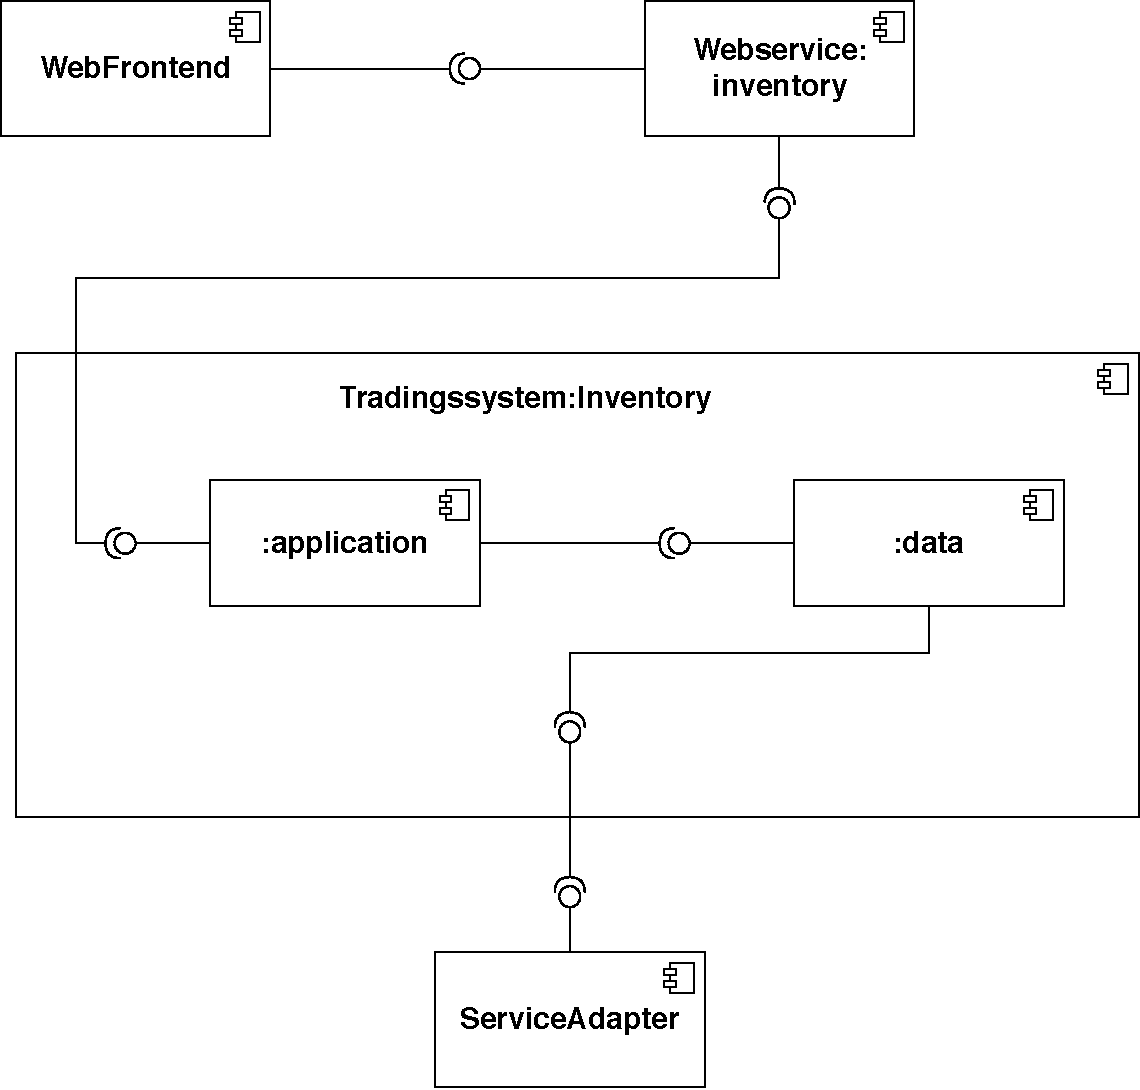
\includegraphics[scale=0.8]{logos/ExcerptUC13.pdf}
\caption{Excerpt of CoCoME for which the described scenarios are defined.}
\label{scn_excerpt}
\end{figure}
\section{Scenario: stock manager requests the report for a customer}
\label{descripScn_casestudy_scn1} 
\subsection{Description}
%\subsubsection{data used in the scenario}
This scenario is derived from the use cases described in the CoCoME tech report \cite{CoCoMETechReport}, more explicit the use case 13. \\
In this scenario, the \textit{StockManager} is already authenticated and then requests a report for the purchased products of a customer. To identify the customer among all customers, the \textit{StockManager} has access to the ID of the specific customer. The \textit{StockManager} enters the ID in CoCoME, then the request is processed. At the end, the stock manager is presented with a full report for the customer. This report contains all purchased products of the customer.
\subsection{Extract the data types, access rights and types of data processing for the scenario} 
\label{accesscontrol_casestudy}
%TODO in drei Schritte aufteilen, erst die verwendeten daten, danch die AR dan ToDP 
In this section, we will first determine what actual data will be used in each component. Next, we obtain the corresponding parts of the two matrices for access rights (ACM) \autoref{ACM_updated} and data processing (OpM) \autoref{typeMatrix}.\\
As stated in the milestone, the data is divided into four classes: customer data, account data, product\&sales data and system data. In the following enumeration for each data class the used data in the scenario is described.
\begin{itemize}
\item account data \\ No data from this class is used in this scenario.
\item customer data\\ The ID from the customer is part of the scenario.
\item product\&sales data\\ In the scenario two data types are used. First, the \textit{IOrderEntries} are used. The \textit{IOrderEntries} are a collection of all data that is generated after an order successful passed.  The second used data type is the \textit{Report} data type, which is a human readable string. 
\item system data \\ This class provides the data that is used to create the queries to the underlying database.
\end{itemize}

Int he next step, we extract the corresponding parts of the ACM and the OpM. The ACM for this scenario is shown in \autoref{accessrightsCSS} and the OpM is shown in \autoref{DataPRoc_UC13}. We omitted the Webservice component for the fact that it only transmits the data.\\
\begin{table}
\begin{tabular}{|c|c|c|c|}
\hline
ACM & Webfrontend & TS:inv:application:store & TS:inv:data:store \\
\hline
stockmanager &
\begin{tabular}{c} 
customer data : 4 \\
account data : 3 \\
p\& s data : 2 \\
system data: 4\\
\end{tabular}
&
\begin{tabular}{c} 
account : 3 \\
customer : 4 \\
product \& sales : 2 \\
\end{tabular}
&
\begin{tabular}{c} 
account : 3 \\\autoref{scn_excerpt})
customer : 4 \\
product \& sales : 2 \\
\end{tabular}
\\
\hline
\end{tabular}
\caption{An ACM showing the access rights for the case study system.}
\label{accessrightsCSS}
\end{table}

\begin{table}
\begin{tabular}{|c|c|c|c|}
\hline 
Types of data & customer data & p\&s data & system data \\
 processing & & & \\
\hline 
Webfrontend & transmit & I/O operations, transmit & non-existent \\ 
\hline 
TS:inv:application & alter, transmit & alter & non-existent \\ 
\hline 
TS:inv:data & relational algebra & relational algebra & alter \\ 
\hline 
\end{tabular} 
\caption{A matrix showing the data processing for each component. the abbreviate p\& s data stands for product and sales data.}
\label{DataPRoc_UC13}
\end{table}

\subsection{Component behavior}
%SEFF  specification
The excerpt of the system model of CoCoME in which the scenario is located is extended with \textit{operations}. For each component one or more operations are defined. These model the data processing in this component. An operation is associated with one of the data processing classes in the OpM \autoref{DataPRoc_UC13}. Each operation has one or more inputs and one more outputs. For each input and each output the data types are known. \\
First, we describe the observable behavior of the scenario across all components and the data processing for each component. All operations are then combined in a data flow.
\subsubsection{Observable Behavior}
%TODO hier weiter machen
%TODO noch genauere Komps
In the scenario, the \textit{StockManager} interacts with CoCoME by requesting a report for a customer. In the following, the behavior of the system  is described.\\
The \textit{StockManager} enters the \textit{ID} of a customer through the \textit{Webfrontend} into CoCoME. The \textit{Webfrontend} processes the ID by transmitting it to the \textit{Webservice} component, which also transmitting the \textit{ID} to the \textit{Tradingssystem:inventory} component. The \textit{Tradingsystem:invetory} consists of two sub components. First, the \textit{ID} is transmitted to the \textit{Tradingsystem:inventory:application:store}, where it is further transmitted to the \textit{Tradingsystem:inventory:data:store} component. In this component a \textit{query} is created by using the \textit{ID}. This query is then send to the \textit{ServiceAdapter}, where the database is requested. The query first selects the respective customer for the \textit{ID}. Then it projects all \textit{IOrderEntries}. The \textit{IOrderEntries} represents an order for a customer. In the \textit{IOrderEntries}, beside other data, which occur with an order, the purchased products are included. The list of all \textit{IOrderEntries} is then transmitted back to the \textit{Tradingssystem:inventory:data:store} and then on to the \textit{Tradingsystem:inventory:application:store}. In this component, the list is then processed in a \textit{Report}. This \textit{Report} is then transmitted via the \textit{Webservice} back to the \textit{Webfrontend}, where the result is shown to the \textit{StockManager}. The resulting report contains a list of all purchased products. In addition, to each entry the date of purchase is added.
\subsubsection{Data flow definition}
Once the general behavior of the scenario within the system has been described, the data flow is created. For each component, the operations and processed data that are used are identified and added to the current component. The operations are then linked in the correct order to complete the creation of the data flow.\\
The overview which data and which operations is shown in \autoref{tab:overview_UC13_DF}.
\begin{table}
\begin{tabular}{|c|c|c|}
\hline 
Components & Operations & Data \\ 
\hline 
Webfrontend & transmit & I: ID  \\
& & II: Report \\
\hline 
Webservice & transmit & I: ID \\ 
& & II: Report \\ 
\hline 
TS:inv:data:store & rel. Algebra & IV: query \\ 
\hline 
TS:inv:app:store & transmit & I: ID  \\ 
& alter data & II: List<IOrderEntries>  \\
\hline 
\end{tabular} 
\caption{Overview over the used operations and the used data for the Scenario: StockManager requests a report for a customer. \textbf{I}}
\label{tab:overview_UC13_DF}
\end{table}
In \autoref{tab:overview_UC13_DF} the association between the components, the used operations and the data is shown. To give a brief explanation of how to read this table. In line 1, the \textit{Webfrontend} only uses the operation \textbf{transmit} and data from a total of 2 classes,  \textbf{customer} data and the \textbf{product\&sales} data. From these classes the concrete data \textit{ID} and \textit{Report} are used.\\
The resulting data flow is shown in \autoref{fig:uc13DFD}.The data flow notation has been extended to include the corresponding component and operations for the processes. The data is still on the edges. Also nothing has changed for the entities.\\
In this scenario a violation for the customer's privacy is displayed. According to the defined access rights tow violations are modeled. First, the \textit{StockManager} should not have access to the \textit{ID} of a customer. And secondly, the \textit{Report} is in combination with the \textit{ID} security relevant. This  data flow should normally prohibited by the system.
%TODO nochmal kurz den Datenfluss beschreiben 
\section{Scenario: Support employee requests information for an order}
This scenario was not defined on the basis of an use case. We defined this scenario for various reasons. First, we wanted to define a counterpart to the already existing scenario (\autoref{descripScn_casestudy_scn1}). The scenario is located in the same system part and therefore operates on the same components. The idea behind this is to provide a violation and a non-violation. An data-based privacy approach my be evaluated by checking if the violation and the non-violation is identified correctly. Due to the fact that CoCoME is a rather minimal system for the goal the system aims for, we couldn't find further use cases where multiple classes of data and/or multiple roles are involved.
\subsection{Description}
\label{scn2_ch4}
The fundamental setting of this scenario is that a customer has a problem with an issued order. To solve the problem, the customer authenticates himself in CoCoME and issues a ticket for the order. The support employee then request a report for the particular order from CoCoME. After the report is presented to the support employee, the scenario has ended. With the report at hand, the support employee should be able to solve the customer's issue.\\

\subsection{Description of a new use case}
We decided to add the scenario described in \autoref{scn2_ch4} as a new use case to CoCoME. The embedding in the already present use cases can be seen in \autoref{UCD_new}.  First we briefly describe the new role added to CoCoME, then the new use case is described.
\begin{figure}
\caption{Use case diagram for CoCoME with the addition of the new use case.}
\label{UCD_new}
\end{figure}
\subsubsection{Description the new role: Support employee}
The support employee role processes the tickets issued by customers. A ticket is issued if there are problems with an order. The support employee receives access to the order and checks their current status. Then he takes an appropriate action to solve the issue if possible. The actions are dependent on the actual order. They can reach from resending the order to taking no action, because the customer tries to scam the enterprise.
% Das nochmal besser erklären, die verschiedenen aktionen sin dzu weit gefächert und werden hier nicht betrachtet
\paragraph{Role description}
The support employee is a new role in the system, so we had to define the access rights for this role. It requires data beyond the data it owns itself, this includes customer and product \& sales related data. The role may provide customer and product \& sales related data. It may happen, for example, that an order is changed, because some products are not available and the customer decides to take a similar product. Also customer may used an invalid credit card in the order under investigation and the credit card details are changed.
\paragraph{access rights}
From the description we derived the access rights shown in \autoref{ACM_SE}. To point out the important definitions. The support employee got no access to the Tradingsystem:cashdeskline, because for his tasks s/he does not need to. Also no access to system data as every role. At last no access to the customer related data in the PickupShop to verify , for example, the credit card details with the bank. We omitted the Tradingsystem:cashdeskline for space purposes 
%\begin{landscape}
\begin{table}
\begin{tabular}{|c|c|c|c|c|}
\hline
ACM & Web-  & TS: & TS: & Pickup  \\
 & frontend  & inventory: & inventory & Shop \\
&  & app:store & data:store &  \\
\hline
support & & & &  \\
employee & & & &  \\
&
\begin{tabular}{c} 
account : 2 \\
customer : 1 \\
product \& : 2 \\
sales\\
system : 4 \\
\end{tabular}
&
\begin{tabular}{c} 
account : 2 \\
customer : 1 \\
product \& : 2 \\
sales\\
system : 4 \\
\end{tabular}
&
\begin{tabular}{c} 
account : 4 \\
customer : 4 \\
product \& : 4 \\
sales\\
system : 4\\
\end{tabular}
&
\begin{tabular}{c} 
account : 4 \\
customer : 2 \\
product \& : 4 \\
sales \\
system : 4 \\
\end{tabular}
%&
%\begin{tabular}{c} 
%account : 2 \\
%customer : 1 \\
%product \&  : 2 \\
%sales \\
%system : 4 \\
%\end{tabular}
\\
\hline
\end{tabular}
\caption{Access right for the role \textit{Support employee}. 1 refers to the access right \textit{FullAccess}, 2 refers to the access right \textit{AccessToUsedData}, 3 refers to the access right \textit{AccessToOwnedData}, 4 refers to the access right \textit{Default}.}
\end{table}
\label{ACM_SE}
%\end{landscape}

\subsubsection{Description of use case 14}
\label{decription_uc14}
\begin{itemize}
\item \textit{Brief Description} The system provides the possibility to generate a report for the current status of a customer's order.
\item \textit{Involved actors} customer, support employee
\item \textit{Precondition} the support employee is authenticated.
\item \textit{Trigger} the customer submits a ticket for a certain order.
\item \textit{Post condition} The report for the order was generated and is displayed to the support employee.
\item \textit{Standard process}
\begin{enumerate}
\item The support employee enters the customers identifier and the report identifier to create the report.
\item The report is generated and displayed
\end{enumerate}
\item Alternative or exceptional process
\begin{itemize}
\item in step 2: the order doesn't exist\\
The system sends an error message to the customer.
\item in step 3: order is ready\\
the support employee sends a reminder to the customer to pick up the order.
\end{itemize}
\end{itemize}


\subsection{Extract the data types, access rights and types of data processing for the scenario}
In this section, we will first determine for the scenario what actual data will be used in each component. Next, we obtain the corresponding parts of the two matrices for access rights (ACM) \autoref{ACM_updated} and data processing (OpM) \autoref{typeMatrix}.\\
As stated in the milestone, the data is divided into four classes: customer data, account data, product\&sales data and system data. In the following enumeration for each data class the used data in the scenario is described.
\begin{itemize}
\item account data \\ No data from this class is used in this scenario.
\item customer data\\ The ID from the customer is part of the scenario.
\item product\&sales data\\ In the scenario two data types are used. First, the \textit{IOrderEntries} are used. The \textit{IOrderEntries} are a collection of all data that is generated after an order successful passed. The second used data type is the \textit{Report} data type, which is a human readable string. 
\item system data \\ In this class the data is located provides the queries to the underlying database.
\end{itemize}

Int he next step, we extract the corresponding parts of the ACM and the OpM. The ACM for this scenario is the same as defined in the new scenario and shown in \autoref{ACM_SE},  and the OpM is shown in \autoref{DataPRoc_UC13}. We omitted the Webservice component for the fact that it only transmits the data.\\

\begin{table}
\begin{tabular}{|c|c|c|c|}
\hline 
Types of data & customer data & p\&s data & system data \\
 processing & & & \\
\hline 
Webfrontend & transmit & I/O operations, transmit & non-existent \\ 
\hline 
TS:inv:application & alter, transmit & alter & non-existent \\ 
\hline 
TS:inv:data & relational algebra & relational algebra & alter \\ 
\hline 
\end{tabular} 
\caption{A matrix showing the data processing for each component. the abbreviate p\& s data stands for product and sales data.}
\label{DataPRoc_UC14}
\end{table}

\subsection{Component behavior}
% hier eventuell en repor tin was anderes umbennen
The excerpt of CoCoME  is extended with \textit{operations}. For each component one or more operations are defined. These model the data processing in this component. An operation is associated with one of the data processing classes in the OpM \autoref{DataPRoc_UC14}. Each operation has one or more inputs and one more outputs. For each input and each output the data types are known. \\
First, we describe the observable behavior of the scenario across all components and the data processing for each component. All operations are then combined in a data flow.
\subsubsection{Observable behavior}
In the scenario the \textit{SupportEmployee} requests and receive a report for a specific order of a customer. In the following, the behavior of the system  is described.\\
The \textit{SupportEmployee} enters the \textit{ID} of the customer and the \textit{ID} of the order. Then the tuple is transmitted via the \textit{Webservice} component and the \textit{Tradingsystem:inventory:application:store} component to the \textit{Tradingsystem:inventory:data:store} component. In this component the tuple is utilizied to create a query that is transmitted to the \textit{ServiceAdapter}. In this component the query is executed and the result is transmitted through the \textit{Tradingsystem:inventory:data:store} component to the \textit{Tradingsystem:inventory:application:store} component. There the result of the query is processed into a \textit{Report}. This \textit{Report} is then transmitted via the \textit{Webservice} component to the \textit{Webfrontend}, where it is shown to the \textit{SupportEmployee}. The resulting report contains meta data in addition to the ordered products. This meta data includes, for example, delivery day, the used payment method, etc.


First the ID of the authenticated customer and the ID of the order are entered in the Webfrontend by the support employee. Then the tuple is transmitted through the Webservice to the Tradingsystem:inventory. The Tradingssystem:inventory consists out of two compoents. First, the Tradingssystem:inventory:application transmits the tuple to Tradingssystem:inventory:data, where the tuple stays for the time being. Then the whole database is selected. In the next step, a query is created by using the customer ID. Then the query is used to select the corresponding customer. Then order ID is used to build another query and select the corresponding order. The order and the customer data is passed to the Tradingsystem:inventory:application, where it is processed to create an report. This report contains meta data in addition to the ordered products. This meta data includes,for example , the day of delivery, the payment method used, etc. Then the report is transmitted via the Webservice component back to the Webfrontend. There the report is shown to the support employee.
\subsubsection{Data flow definition}
Previously, the data was divided into equivalence classes.  Now we present the concrete data to be used in this scenario and specify the corresponding classes.\\
%TODO datenklassen hinzufügen
\begin{itemize}
\item Webfrontend\\ Transmit the (customer ID (customer data), order ID (product\& sales related data)) tuple and the resulting report (product\& sales related data).
\item Tradingsystem:inventory:application \\ Transmits the tuple and alters the Customer and Order object to a report and transmits it.
\item Tradingsystem:inventory:data \\ Transmit the Customer and Order object and takes the tuple to create two queries.
\end{itemize}
With these informations about the data processing, we are able to build the resulting data flow, which is shown in \autoref{DF_UC14}.

\begin{figure}
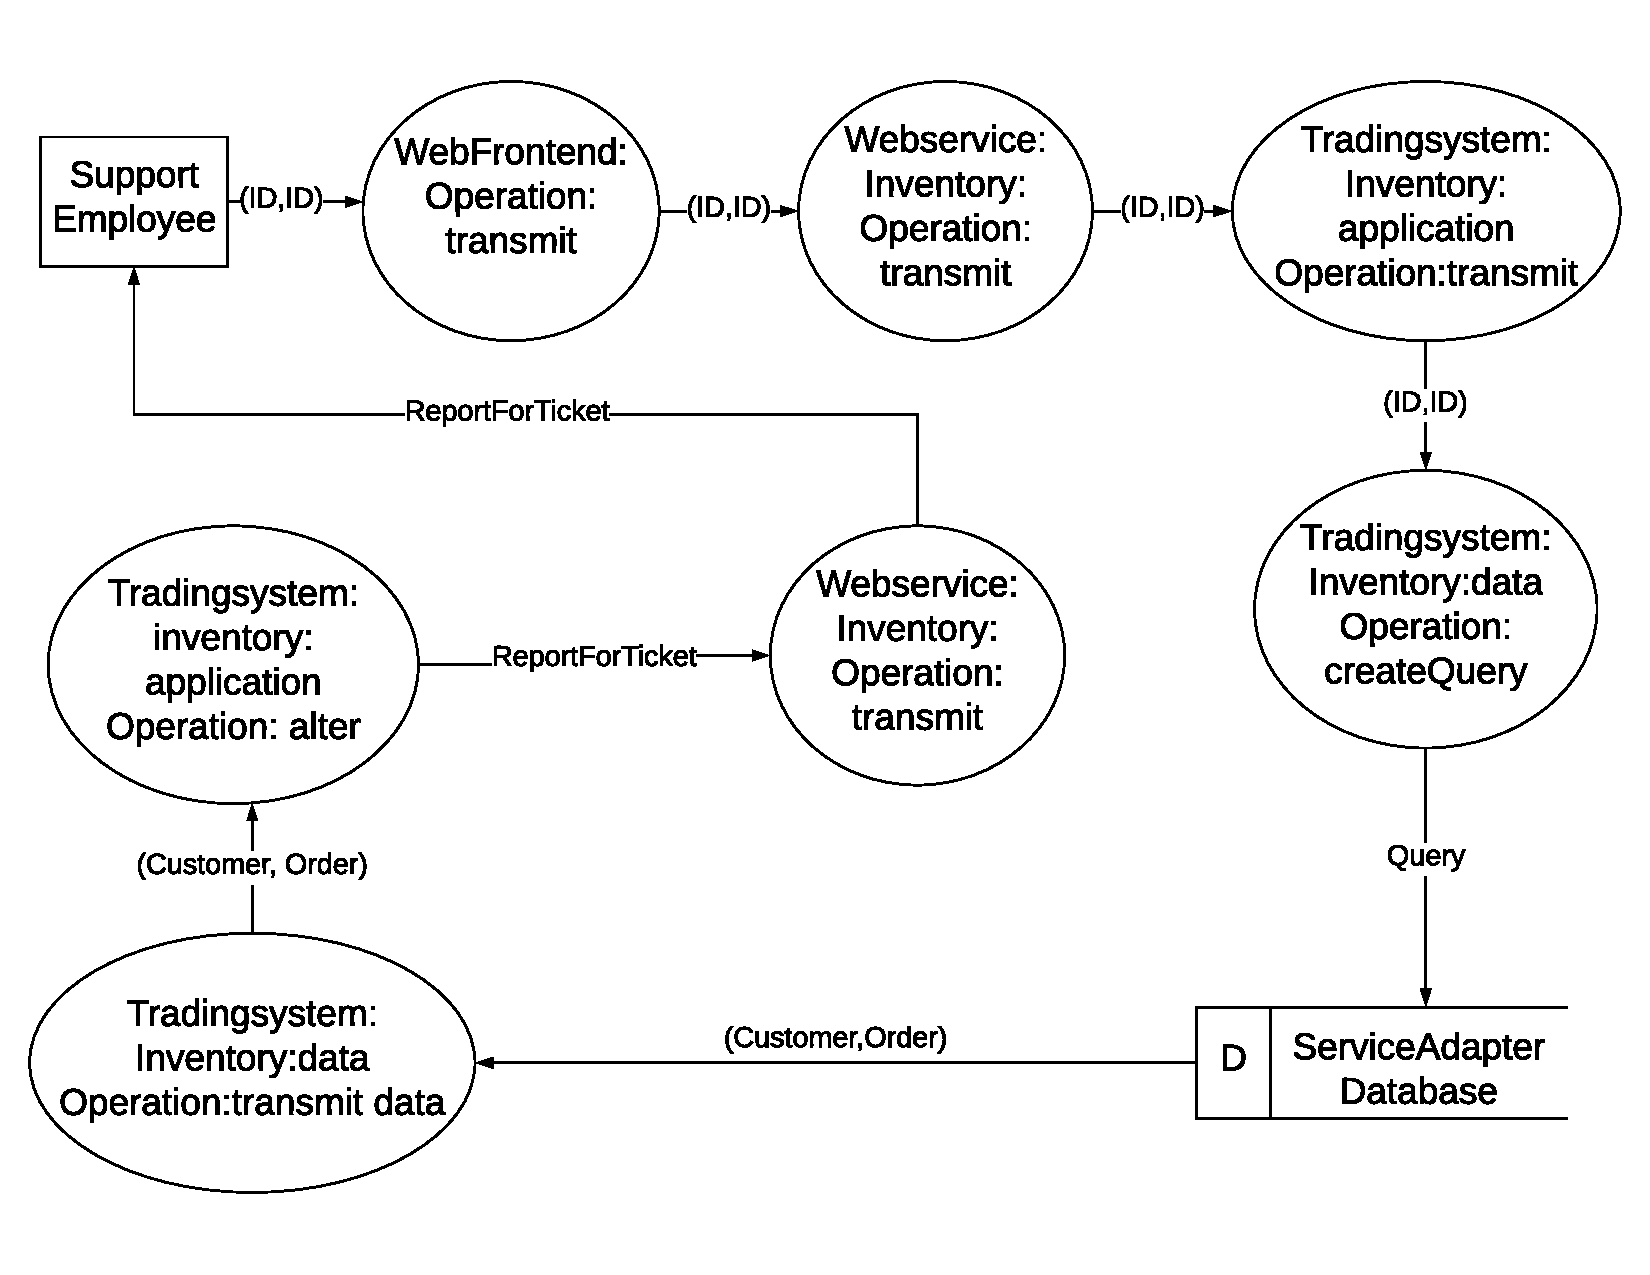
\includegraphics[scale=0.8, angle = 90]{logos/DF_UC14.pdf}
\caption{The resulting data flow for the scenario: Support employee requests information for an order.}
\label{DF_UC14}
\end{figure}
\section{Evaluation of the scenarios}
After all data flow are defined and added to the system, the second part of the evalaution for the case study is conducted in this section. The overview is shown in \autoref{Overview_CSS_Eval}. 
\begin{figure}
\caption{Overview for the evaluation for the \nameref{ch:casestudysystem}}
\label{Overview_CSS_Eval}
\end{figure}
\subsection{Goal: Evaluation for the created case study}
The goal is to evaluate the case study. As shown in \autoref{Overview_CSS_Eval} the evaluation of the case study is split into two parts. In this we will only focus on the highlighted plan, the evaluation of the defined scenarios.
\subsection{Question: Is the case study usable for a data-based privacy analysis?}
To verify if the created case study are usable for the evaluation of a data-based privacy analysis, it is checked which information flow classes the created case study covers. We relied on the problem statement \textit{Non-influence} \cite{Noninfluence}. Non-influence combines two sub problem statements, \textit{Non-interference} and \textit{Non-leakage}. Non-inference describes that no role may acquire information from a role that inherits a higher security level. In the course of a program flow, user with a high security level and user with low security level inserts data in the system and receive outputs from the system. If there is no interference in the system, inputs from high level user have no effect to the outputs of low level user. The effects of \textit{Non-inteference} can be expressed by three infromtion flow classes: \textbf{Illegal information flow}, \textbf{Direct information flow between roles} and \textbf{Information flow form high to low}. \\
Illegal information flow describes that a role can receive information for which it is not authorized.\\
Direct information flow describes the flow of information between two roles for which  is not cleared to either receive or transmit.\\
Information from high to low describes flow of information, even if not intended, from a higher security level to a lower security level.
\textit{Non-leakage} describes the issue that it is not observable what specific actions are taken place by a system. This can be expressed by the information flow class \textbf{Observable information flow}.\\
The metric is the number of covered information flow classes in the case study. The evaluation is conducted in a checklist manner. 

\subsubsection{Number of different covered information flow classes}
We evaluate the variety of covered information flow classes for the defined scenarios in the case study. We defined four information flow classes to cover \textit{Non-influence}(\textit{non-interference} + \textit{non-leakage}. The covered information flow classes are: Illegal information flow, information flow from higher security levels to lower ones, observable information flow and direct information flow between roles. W
\paragraph{Illegal information flow}
The first scenario covers illegal data flow. The stock manager in this scenario has access to the \textit{ID} of an customer. The role has no rights to have access \textit{customer} data. Then, the stock manager request a report of this specific customer and receives a full report for this customer. The stock manager has the security level \textit{AccessToUSedData}. The report for one customer is no necessary data for the stock manager to perform its tasks. In this scenario an illegal data flow is modeled. Therefore, the illegal data flow class is part of the created case study.
\paragraph{Information flow from high to low}
In the defined scenarios, for the role involved, data from different security levels is present. The data associated also flows to lower levels. This information flow class is also covered.
\paragraph{Direct information flow between roles} For the fact that no scenario with more than one role is defined, this class is also not covered in the case study.
\paragraph{Observable information flow}
This information flow class is not modeled in the scenarios. 
%TODO Tabelle fehlt noch 

\begin{table}
\centering
\begin{tabular}{|c|c|} 
\hline 
Data flow & fulfilled? \\ 
\hline 
Illegal information flow & \cmark \\ 
\hline 
Information flow from high to low & \cmark \\  
\hline 
Direct information flow between roles & \xmark \\ 
\hline 
No observable information  flow & \xmark \\
\hline 
\end{tabular}
\caption{Resulting checklist for the evaluation of the case study.}
\label{Eval_infoFlowClasses}
\end{table}

\section{Discussion}
%TODO general discussion warum dinge so gemacht wurden wie sie gemacht wurden !!!!!
% warum wir die query explizit definiert, warum wurde die DF notation angepasst, 
In this section, we are going to discuss the single design decision that were made during the creation of the case study. Further, we discuss we if the process can be concluded.
